
\section{Introduction}
	Impedance spectroscopy, introduced in \cpageref{characterization_impedance}, is a powerful technique for characterizing electronic devices in the frequency domain.
	The first information that can be directly extracted from impedance spectroscopy is a frequency\hyp{}dependent capacitance \cite{Brus2016}.
	When studying this in perovskite solar cells, the results are of difficult interpretation \cite{Almora2018,Guillen2014}.
	A giant capacitance is always observed at low frequencies for illuminated devices \cite{Juarez-Perez2014,Kim2015c}.
	More rarely, also a negative capacitance (\textsl{i.e.} an inductance) has been observed in perovskite solar cell \cite{Ghahremanirad2017,Guerrero2016,Sanchez2014} and other kinds of solar cells \cite{Mora-Sero2006,Knapp2015}.
	In order to extract the individual parameters, like transport and recombination constants, the data has to be fitted using an electronic equivalent circuit \cite{Jamnik2001}.
	The components of the circuit should have a relation with the actually existing processes, so that we can relate the parameters of the electrical component with the solar cell specific internal mechanisms.
	Many complex circuits have been proposed in literature, some of them included inductors for matching the inductive behaviour \cite{Almora2018,Ghahremanirad2017,Guerrero2016}.
	Previously to our publication, these phenomena were interpreted as caused by a huge free charge accumulation at the interfaces due to the influence of ionic accumulation \cite{Guerrero2016,Zarazua2016a} supported by drift\hyp{}diffusion simulations \cite{Garcia-Rosell2018,Lopez-Varo2018}.
	It has to be noted that any slow process causing a change in the flowing current could result in an apparent capacitance or inductance, this could happen with degradation processes or heating \cite{Knapp2015}.
	In perovskite solar cells, the electrostatic potential arising from mobile ion redistribution controls electronic charge transfer barriers \cite{Tress2016,Pockett2017}.
	In May 2018 we uploaded to ArXiv a pre-print which was then published in \authoryear{Moia2019} with an alternative interpretation for the giant capacitance: this influence of the ionic charge on the electronic processes such as recombination and can give rise to apparent capacitive behaviour.
	This effect does not involve an accumulation of an enormous amount of charge, as it was expected by a giant capacitance, so it cannot be described by a capacitor in the equivalent electrical circuit.
	For the inductive behaviour we proposed that the same influence can affect the charge injection causing a negative apparent capacitance.
	More or less at the same time, other research groups published similar interpretations \cite{Ebadi2019,Jacobs2018}.
	We proposed that both of the effects (apparent capacitance and inductance) can be described by transistors element in the circuit, as represented in \cref{fig:diode_transistor-transistor}.
	This allows the charge to flow through an interface to not only depend on the applied voltage, like in a common diode, but also on an external influence: the ionic density close to the interface.
	The influence of ionic migration on electronic transfer can be thought as an amplification of electronic current by ionic current.
	Our model not only works in the small perturbation regime employed in impedance spectroscopy, but can also explain data from hysteretic current\hyp{}voltage sweeps.
	The understanding of this mechanism not only allows the researcher to successfully use impedance spectroscopy on perovskite solar cells and other ionic and electronic interfaces (e.g. electrochemical communication between neurons in the brain \cite{Cole1956}) but could also be employed for designing new physical electronic components showing large and tunable apparent capacitance or inductance in a reduced volume.

	\paragraph{Design of the Experiment}
	Impedance spectroscopy has been initially modelled studying the current evolution after a single voltage step.
	This first rough attempt should be polished using Kramers\hyp{}Kronig relation and has not been published yet.
	In order to confirm the initial observations, the impedance spectroscopy has been implemented trying to match the actual experimental conditions.
	For this reason, the oscillating current obtained when applying an oscillating voltage has been studied separately for each frequency.
	This caused the simulation to be much slower but still doable with my laptop.
	Additionally, the phase and amplitude has been obtained mimicking the demodulation of a lock-in amplifier rather than with a sinusoidal fitting.

	\paragraph{Author contributions}
	I implemented and run the impedance spectroscopy simulation on top of Driftfusion software developed by Dr.\ Phil Calado, Dr.\ Piers RF Barnes, Mohammed Azzouzi, Benjamin Hilton, and myself.
	Dr.\ Davide Moia and Dr.\ Piers RF Barnes created the formalism and the electrical equivalent circuit.
	William Fisher and Dr. Davide Moia fitted the experimental data using fitting routines developed by Dr.\ Piers RF Barnes.
	Dr.\ Michael Stringer, Dr.\ Onkar Game, Yinghong Hu, Dr.\ David Lidzey, and Dr.\ Pablo Docampo provided excellently stable perovskite solar cells to be studied.

\section{Driftfusion software}
	Driftfusion is a modelling platform for stacked semiconductors, mostly used for solar cells.
	It estimates the profile of electrostatic potential, free electrons, free holes, and mobile ions densities over one dimension (depth into the stack) and over time.
	The semi-classical transport, continuity, and Poisson's equations are solved using Matlab's built-in Partial Differential Equation solver for Parabolic and Elliptic equations \texttt{pdepe}
	The simulation assumes static negative counter ions simulating Schottky defects \cite{Walsh2015} and positively charged mobile ions constrained into the absorber layer.
	This formalism is based on \authoryear{Nelson2003} and described in \authoryear{Calado2016} and \authoryear{Calado2018}.
	All the mentioned functions, helper code and examples of impedance spectroscopy simulations have been released on \url{https://github.com/barnesgroupICL/Driftfusion/tree/2018-EIS}.

	\paragraph{Homojunction}
	I employed an homojunction version of Driftfusion, which at the date of September 2017 was the stable and well tested release of Driftfusion.
	This means that in the presented simulations all the materials have the same band gap but can differ by other parameters: doping level (equilibrium Fermi level position), holes and electrons mobilities, permittivity, radiative and trap mediated recombination constants, traps relative energy inside the band gap, and thickness.
	This proved to be enough for simulating the influence of ionic current on the recombination current but was limited for studying their influence on the injection current.

	\paragraph{Recombination and generation}
	High rates of recombination in the contact regions are used to simulate surface recombination.
	Even if an optical model was available in Driftfusion, an uniform generation through all the absorber proven to be enough for our purposes.



	\paragraph{Boundary conditions}
	The oscillating voltage is applied with time\hyp{}dependent boundary conditions.

\section{Simulating impedance spectroscopy}

	\paragraph{Initial conditions}
	The solution of the charge and electrostatic concentration profiles of the device under steady state operating conditions was determined using Driftfusion core functions to provide initial conditions for the simulated impedance spectroscopy.
	Most importantly, the illumination intensity and the DC voltage $\bar V$ which are the usually explored parameters in each complete simulation.

	\paragraph{Applied voltage}
	The impedance spectroscopy simulations were performed by applying an oscillating voltage $v$ superimposed on a background bias voltage $\bar V$ boundary condition:

	\begin{equation}
		V = \bar V + v(t) = \bar V + v_|max| \sin(\omega t)
	\end{equation}

	Usually, a $v_|max|$ of \SI{2}{\mV} is employed.
	This value is much smaller than the experimentally used one but very similar results are obtained when using larger perturbations (simulations with a $v_|max|$ of \SI{200}{\mV} are mentioned in \cpageref{impedance-large_perturbations}).
	The small value allowed me to obtain a computationally fast simulation without being affected by too much numerical noise.

	\paragraph{Position and time grids}
	In order to deal with the high gradients at the interfaces, a linear spatial mesh was used with a spacing of \SI{0.55}{\nm} within the approximate depletion regions of the device and \SI{2.54}{\nm} elsewhere.
	Even if the \texttt{pdepe} solver utilises an internal time grid, it outputs the data at the requested times array.
	All the stabilizations have been performed on a logarithmic time grid (\texttt{tmesh\_type}$=2$ in \texttt{meshgen_t}) while all the oscillating voltage simulations have been performed on a linear time grid (\texttt{tmesh\_type}$=1$ in \texttt{meshgen_t}).
	For the impedance simulations, 20 complete periods are simulated with 40 time points for each period.

	\paragraph{Oscillating stabilization}
	The change from steady state to oscillating voltage does require some complete periods before reaching a stable oscillation (where the current profile is identical from one period to the next).
	As represented in \cref{fig:impedance_flowchart}, before analysing the oscillating solutions, the stabilization is verified comparing the last time point profiles with the profiles at the half of the current simulation (so at the \nth{10} period).
	In case the stability was absent, the last time point solution has been used as a starting point for 20 more periods, until when stabilization was ensured.
	This is mostly important for large perturbation simulations (large $v_|max|$), where the time\hyp{}averaged profiles are rather different from the steady state ones.

	\begin{SCfigure}%demodulation
		\centering
		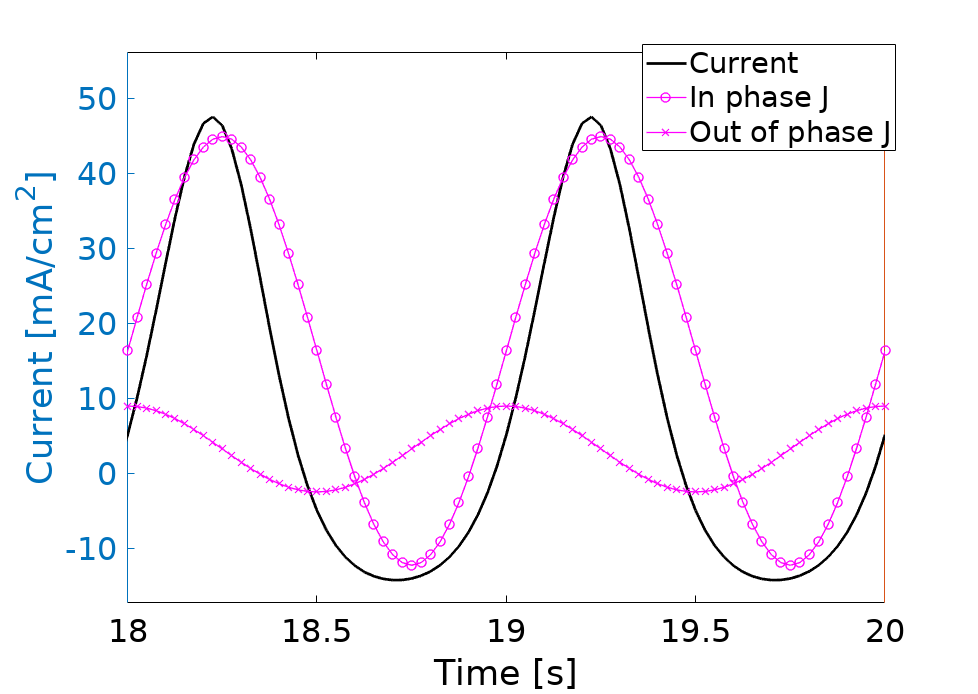
\includegraphics[width=0.65\textwidth]{demodulation/demod-result.png}
		\mycaption[Example of demodulation on a large perturbation simulation.]{
			The applied voltage is not shown, it was a sinusoidal wave with frequency \SI{1}{\Hz}.
			Black line is the simulated oscillating current, the non sinusoidal shape is due to the large amplitude of the applied oscillating voltage.
			Pink lines are the output of the demodulation routine.
		}\label{fig:demodulation}
	\end{SCfigure}

	\paragraph{Demodulation}
	The amplitude and phase of the oscillating electronic current density was obtained via
	demodulation, mimicking the working principle of a two-phase lock-in amplifier \cite{WikipediaLockIn}.
	As can be seen in \cref{fig:demodulation}, this method works both with sinusoidal profiles obtained from small perturbation simulations and also for large perturbation signals including distortion by higher harmonics.
	It has been implemented in \texttt{ISwave\_EA\_single\_demodulation} described in \cpageref{ISwave_EA_single_demodulation}.
	The current density profile $j(t)$ was point-by-point multiplied by the voltage profile or the \SI{90}{\degree} shifted
	voltage profile normalised by $v_|max|$ and integrated over time (typically 10 periods):

	\begin{equation}
		X = \frac{\omega}{m \pi} \int_{t_0}^{t_0+2m\pi / \omega} j(t) \sin(\omega t) \dd t
	\end{equation}

	\begin{equation}
		Y = \frac{\omega}{m \pi} \int_{t_0}^{t_0+2m\pi / \omega} j(t) \cos(\omega t) \dd t
	\end{equation}

	where $m$ is the number of periods, $t_0$ is the start of the integration time, $\sin(\omega t)$ is the normalised voltage profile, and $\cos(\omega t)$ is the \SI{90}{\degree} shifted one.
	Actually, for avoiding numerical problems (\texttt{e.g.} values close to the double limit) the current profile constant bias is subtracted and the result is normalised.
	Amplitude $j_|max|$ and
	phase $\theta$ are then given via:

	\begin{equation}
		j_|max| = \sqrt{X^2 + Y^2}
	\end{equation}

	\begin{equation}
		\theta = \arctan(\frac{Y}{X})
	\end{equation}
	allowing the complex impedance to be determined \textsl{via} $Z = v_|max| / j_|max| \exp(-\mathrm{i}\theta)$.
	The amplitude and phase
	obtained this way were confirmed by fitting j(t) with a sinusoidal function.

	\paragraph{Calculation of Ionic Displacement Current}\label{displacement_current_ionic}
	As seen in \cpageref{intro_displacement_current}

	\mysection[Simulated apparent capacitance]{Simulated apparent capacitance spectra characteristics}

	\begin{figure}%impedance-capacitance
		\makebox[\textwidth][c]{
			\parbox{1.1\textwidth}{
				\centering
				\begin{subfigure}[t]{0.51\textwidth}
					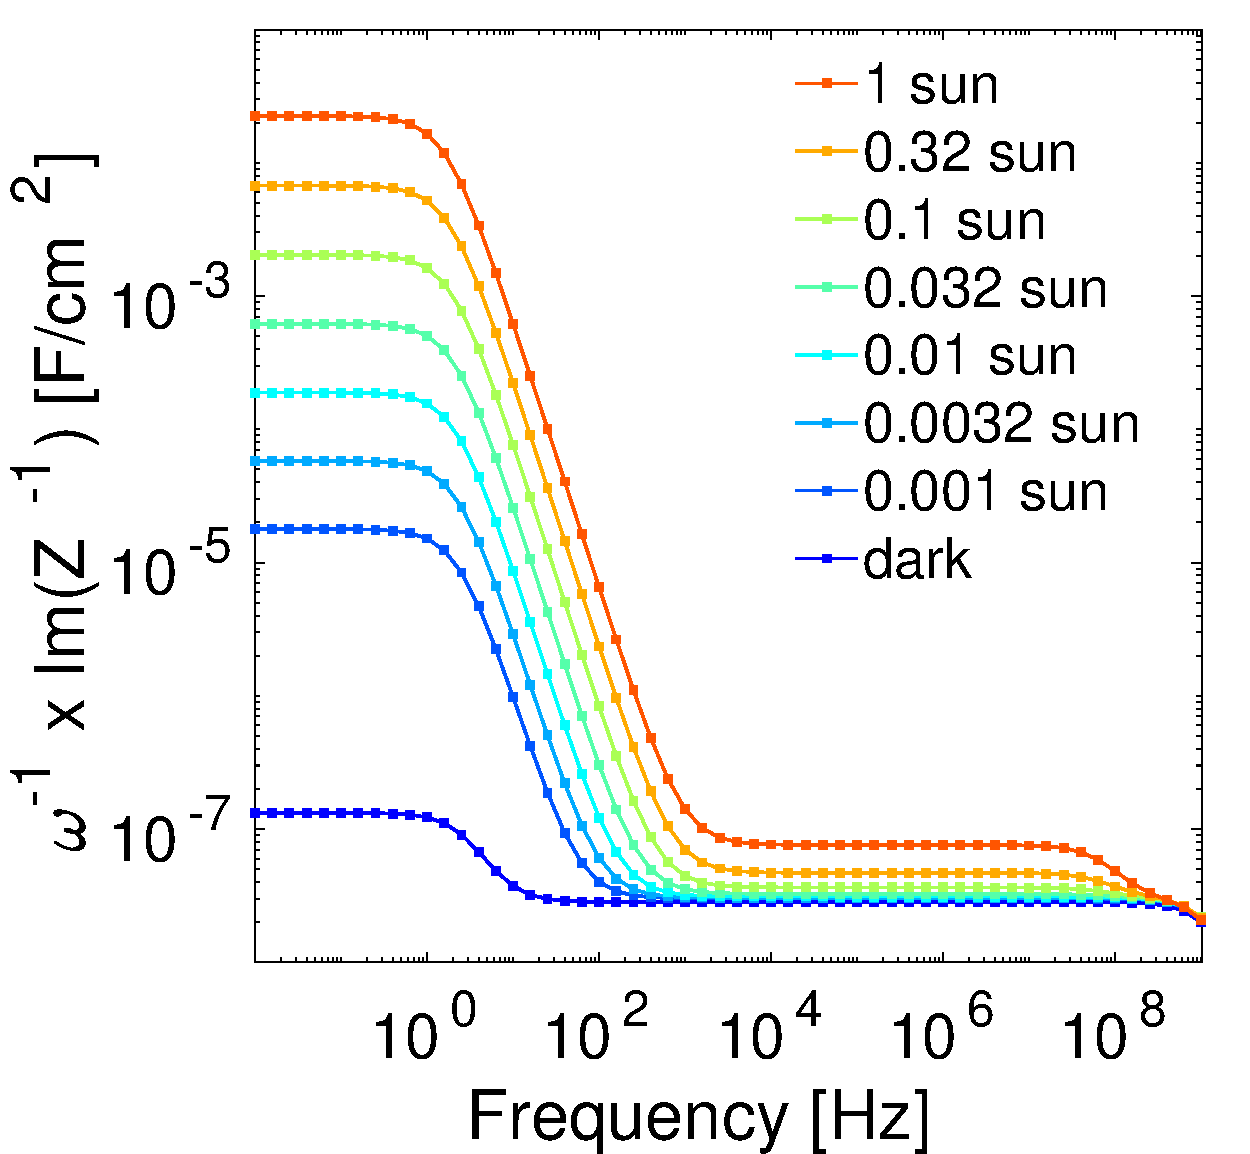
\includegraphics[width=1\textwidth]{dd_capacitance/capacitance-small.pdf}
					\subcaption{Illuminated, open circuit}\label{fig:impedance-capacitance-oc}
				\end{subfigure}
				\qquad
				\begin{subfigure}[t]{0.51\textwidth}
					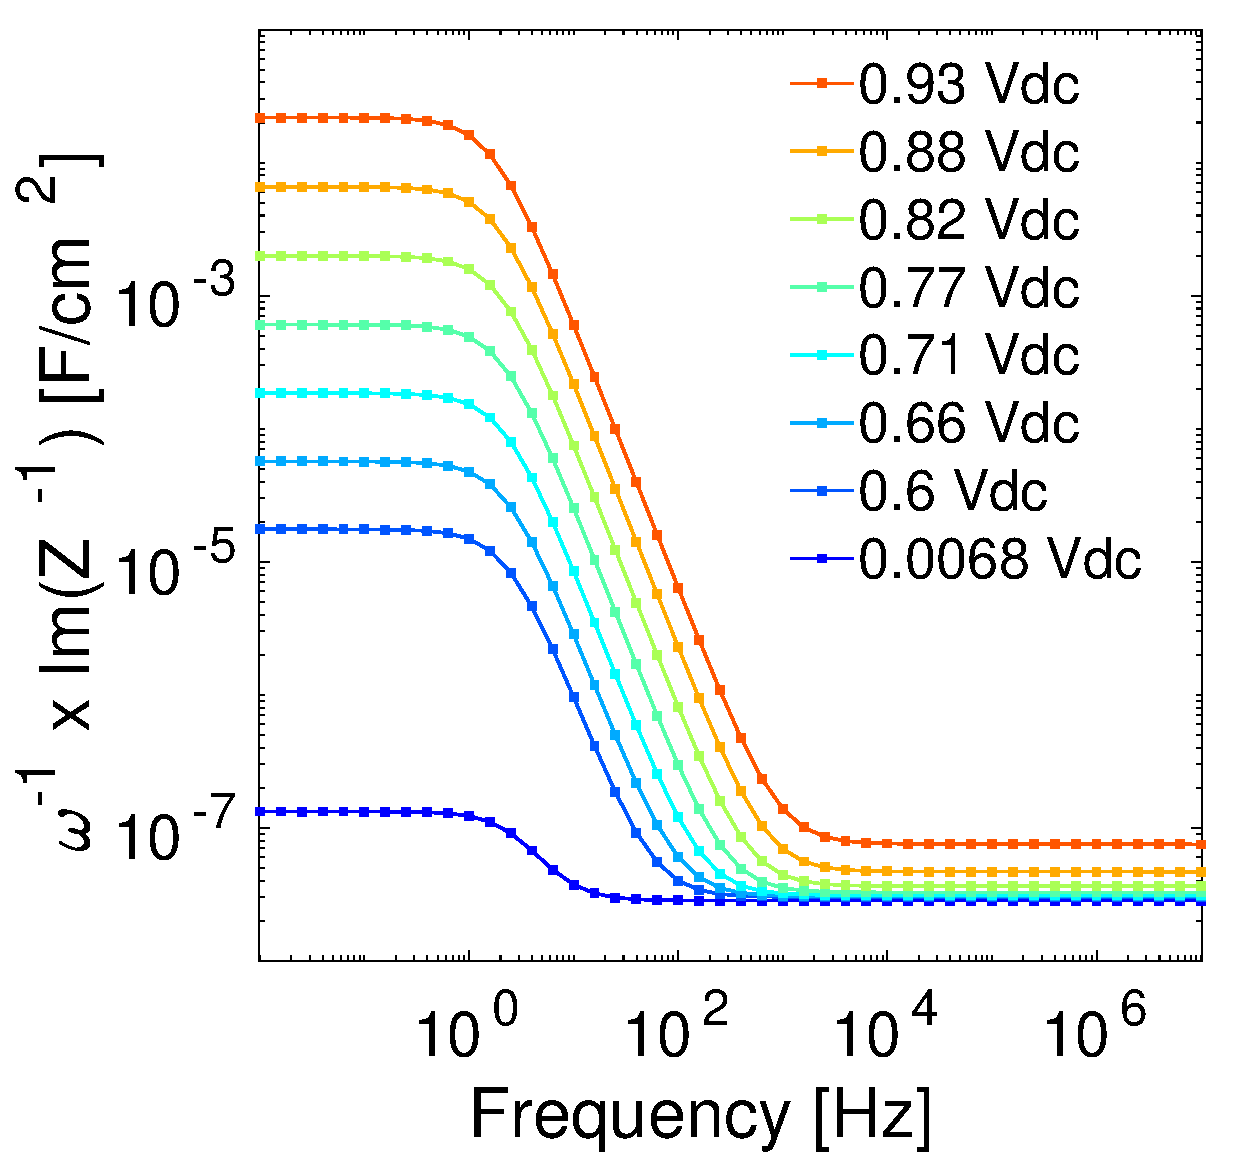
\includegraphics[width=1\textwidth]{dd_capacitance/vapp-cap-small.pdf}
					\subcaption{Dark, applied voltage}\label{fig:impedance-capacitance-vapp}
				\end{subfigure}
				\mycaption[Simulated apparent capacitance spectra of an illuminated perovskite solar cell at open circuit and dark applied voltage.]{
					In (\textbf{a}) the simulation oscillates the voltage around the \gls{voc} value induced by different light intensities at open circuit (light bias).
					In (\textbf{b}) the voltages from (\textbf{a}) are applied as constant voltage biases around which the applied voltage oscillates, in dark.
				}\label{fig:impedance-capacitance}
			}
		}
	\end{figure}

	%\begin{figure}
	%	\centering
	%	\includegraphics[width=1.1\textwidth]{dd_capacitance/capacitance.pdf}
	%	\mycaption[Simulated apparent capacitance spectra of an illuminated perovskite solar cell at open circuit.]{}\label{fig:impedance-capacitance}
	%\end{figure}

	%\subsection{Very high frequency}



	%\subsection{Mid frequency}

	\begin{figure}%impedance-accumulation
		\centering
		\includegraphics[width=1.1\textwidth]{dd_capacitance/accumulation.pdf}
		\mycaption[Simulated accumulation capacitance spectra compared with capacitance due to charge accumulation.]{}\label{fig:impedance-accumulation}
	\end{figure}

	\begin{figure}%cap_scheme_hi_low_freq
		\makebox[\textwidth][c]{
			\parbox{1.1\textwidth}{
				\centering
				\begin{subfigure}[t]{0.51\textwidth}\centering
					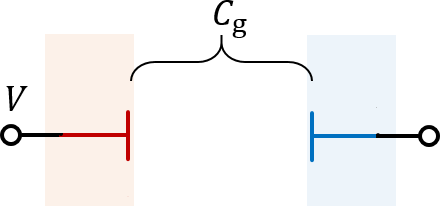
\includegraphics[width=0.8\textwidth]{cap_scheme_hi_low_freq/capacitance_no_ions.png}
					\subcaption{Capacitance at mid frequencies}\label{fig:cap_scheme_hi_freq}
				\end{subfigure}
				\qquad
				\begin{subfigure}[t]{0.51\textwidth}\centering
					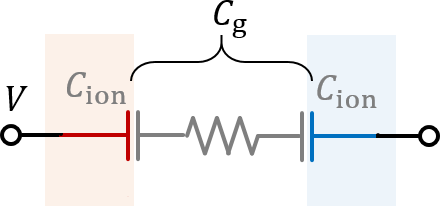
\includegraphics[width=0.8\textwidth]{cap_scheme_hi_low_freq/capacitance_with_ions.png}
					\subcaption{Capacitance at low frequencies}\label{fig:cap_scheme_low_freq}
				\end{subfigure}
				\mycaption[Capacitance representation with or without mobile ions.]{}\label{fig:cap_scheme_hi_low_freq}
			}
		}
	\end{figure}

	%\subsection{Low frequency}

	\begin{figure}%impedance-ionic
		\makebox[\textwidth][c]{
			\parbox{1.1\textwidth}{
				\centering
				\begin{subfigure}[t]{1.1\textwidth}
					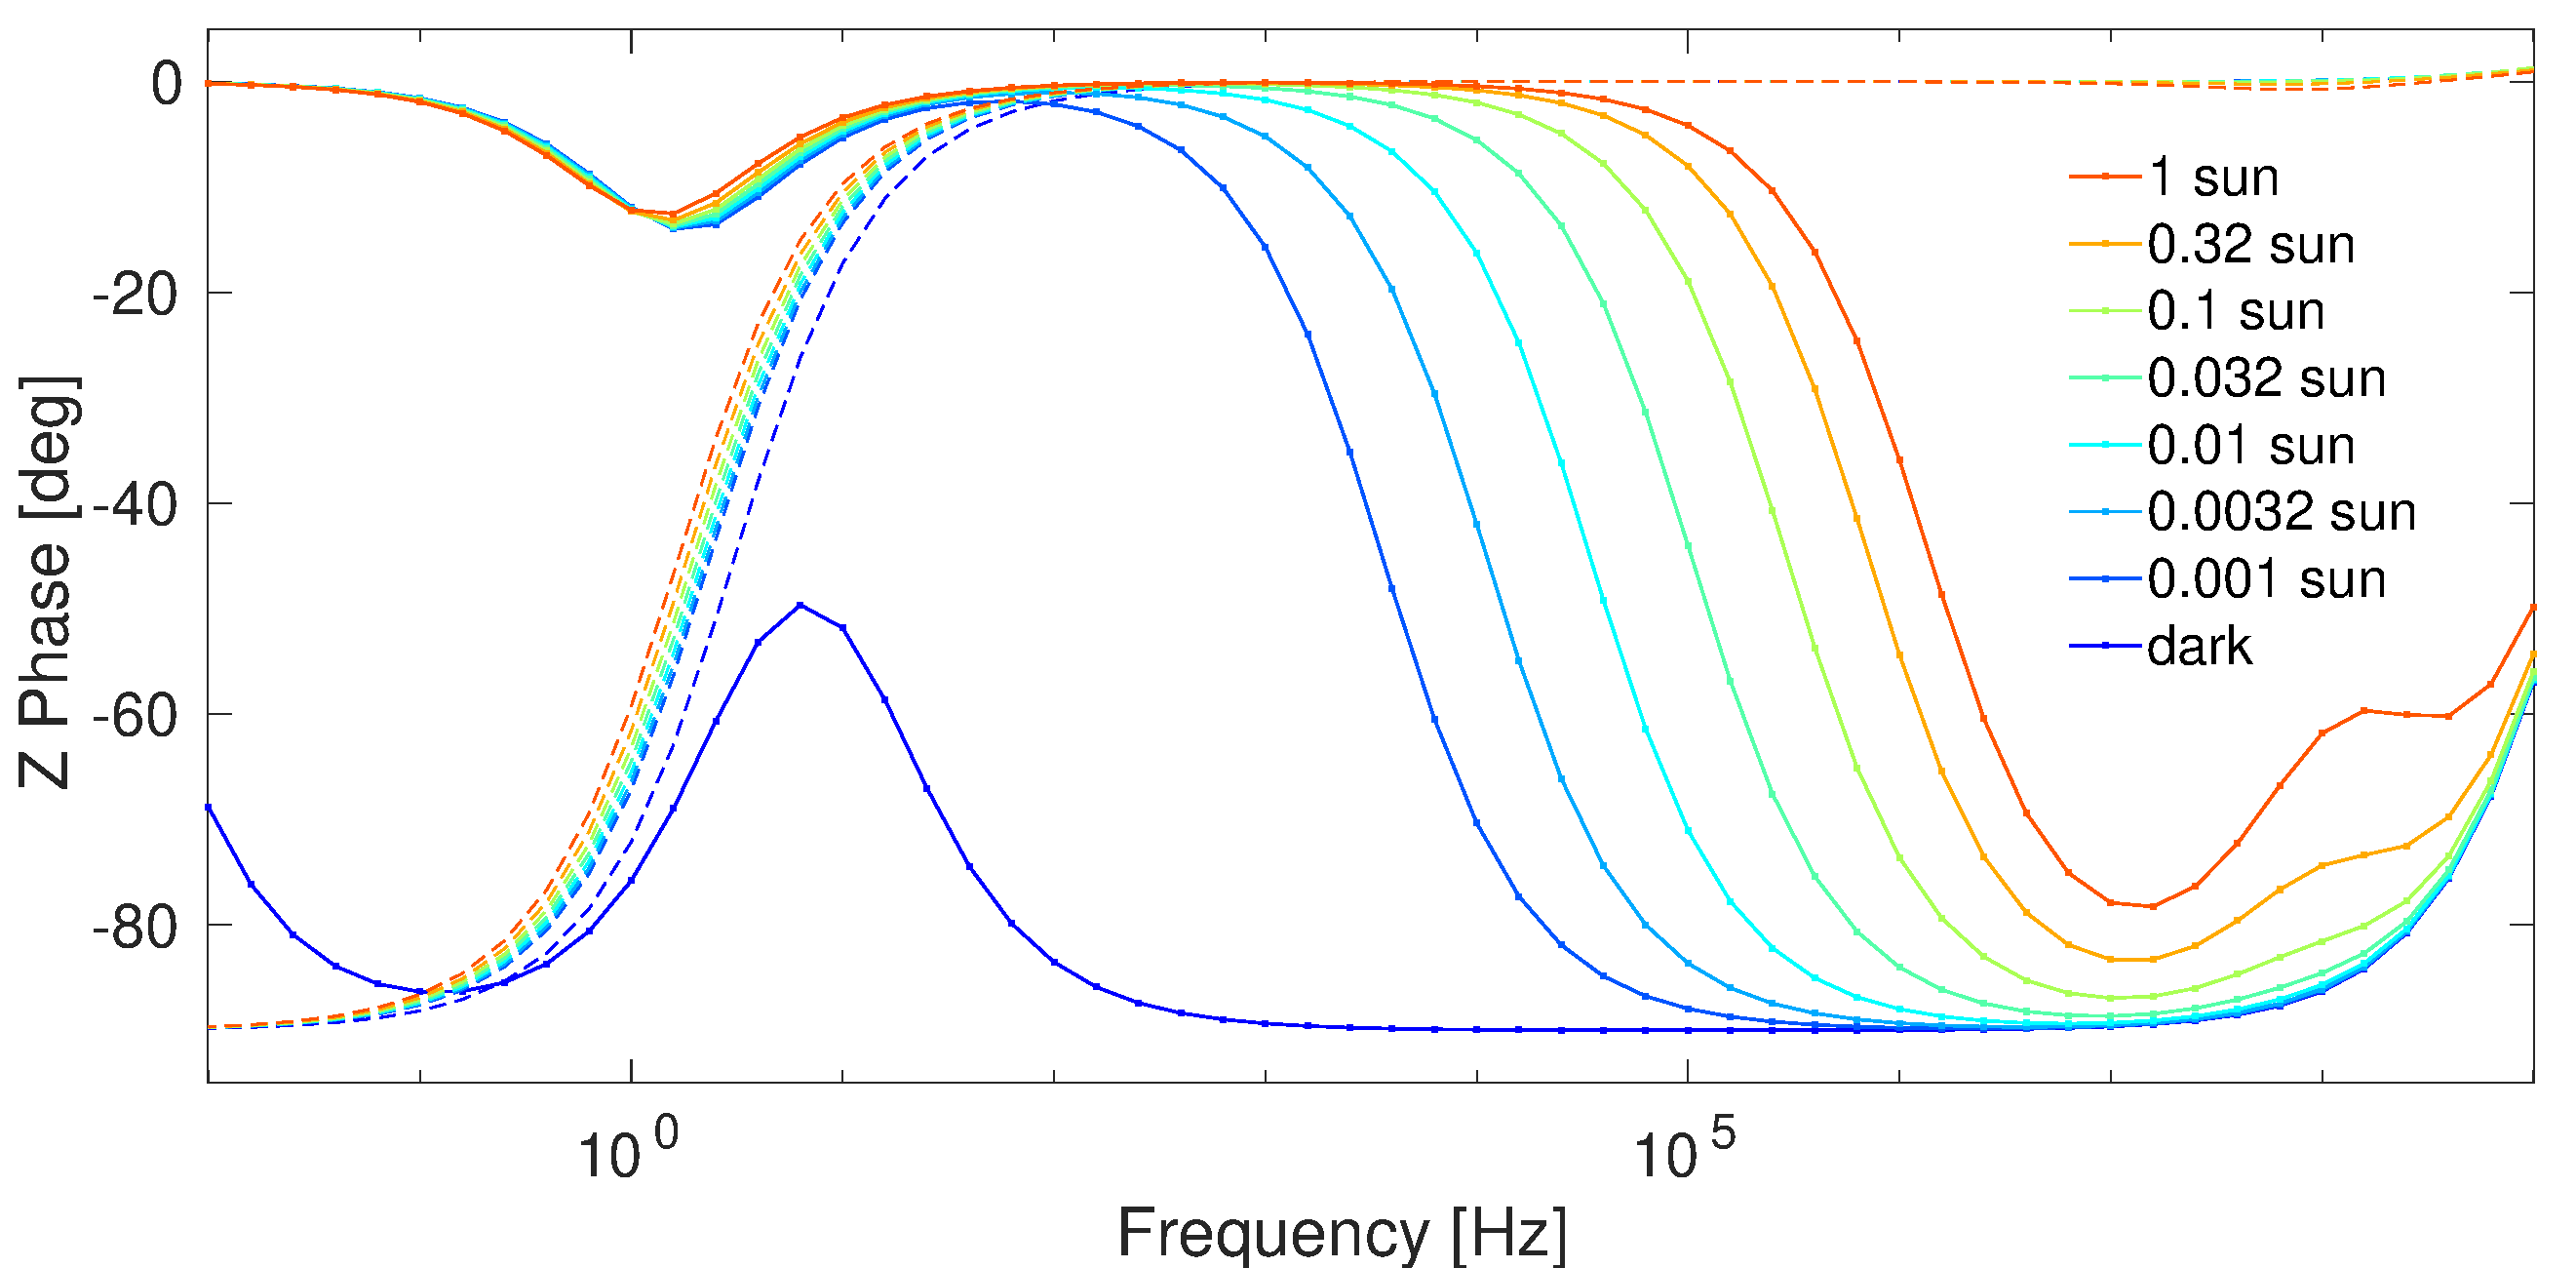
\includegraphics[width=1.05\textwidth]{dd_phase/phase.pdf}
					\subcaption{Ionic displacement current phase}\label{fig:impedance-ionic-phase}
				\end{subfigure}
				\bigskip

				\begin{subfigure}[t]{1.1\textwidth}
					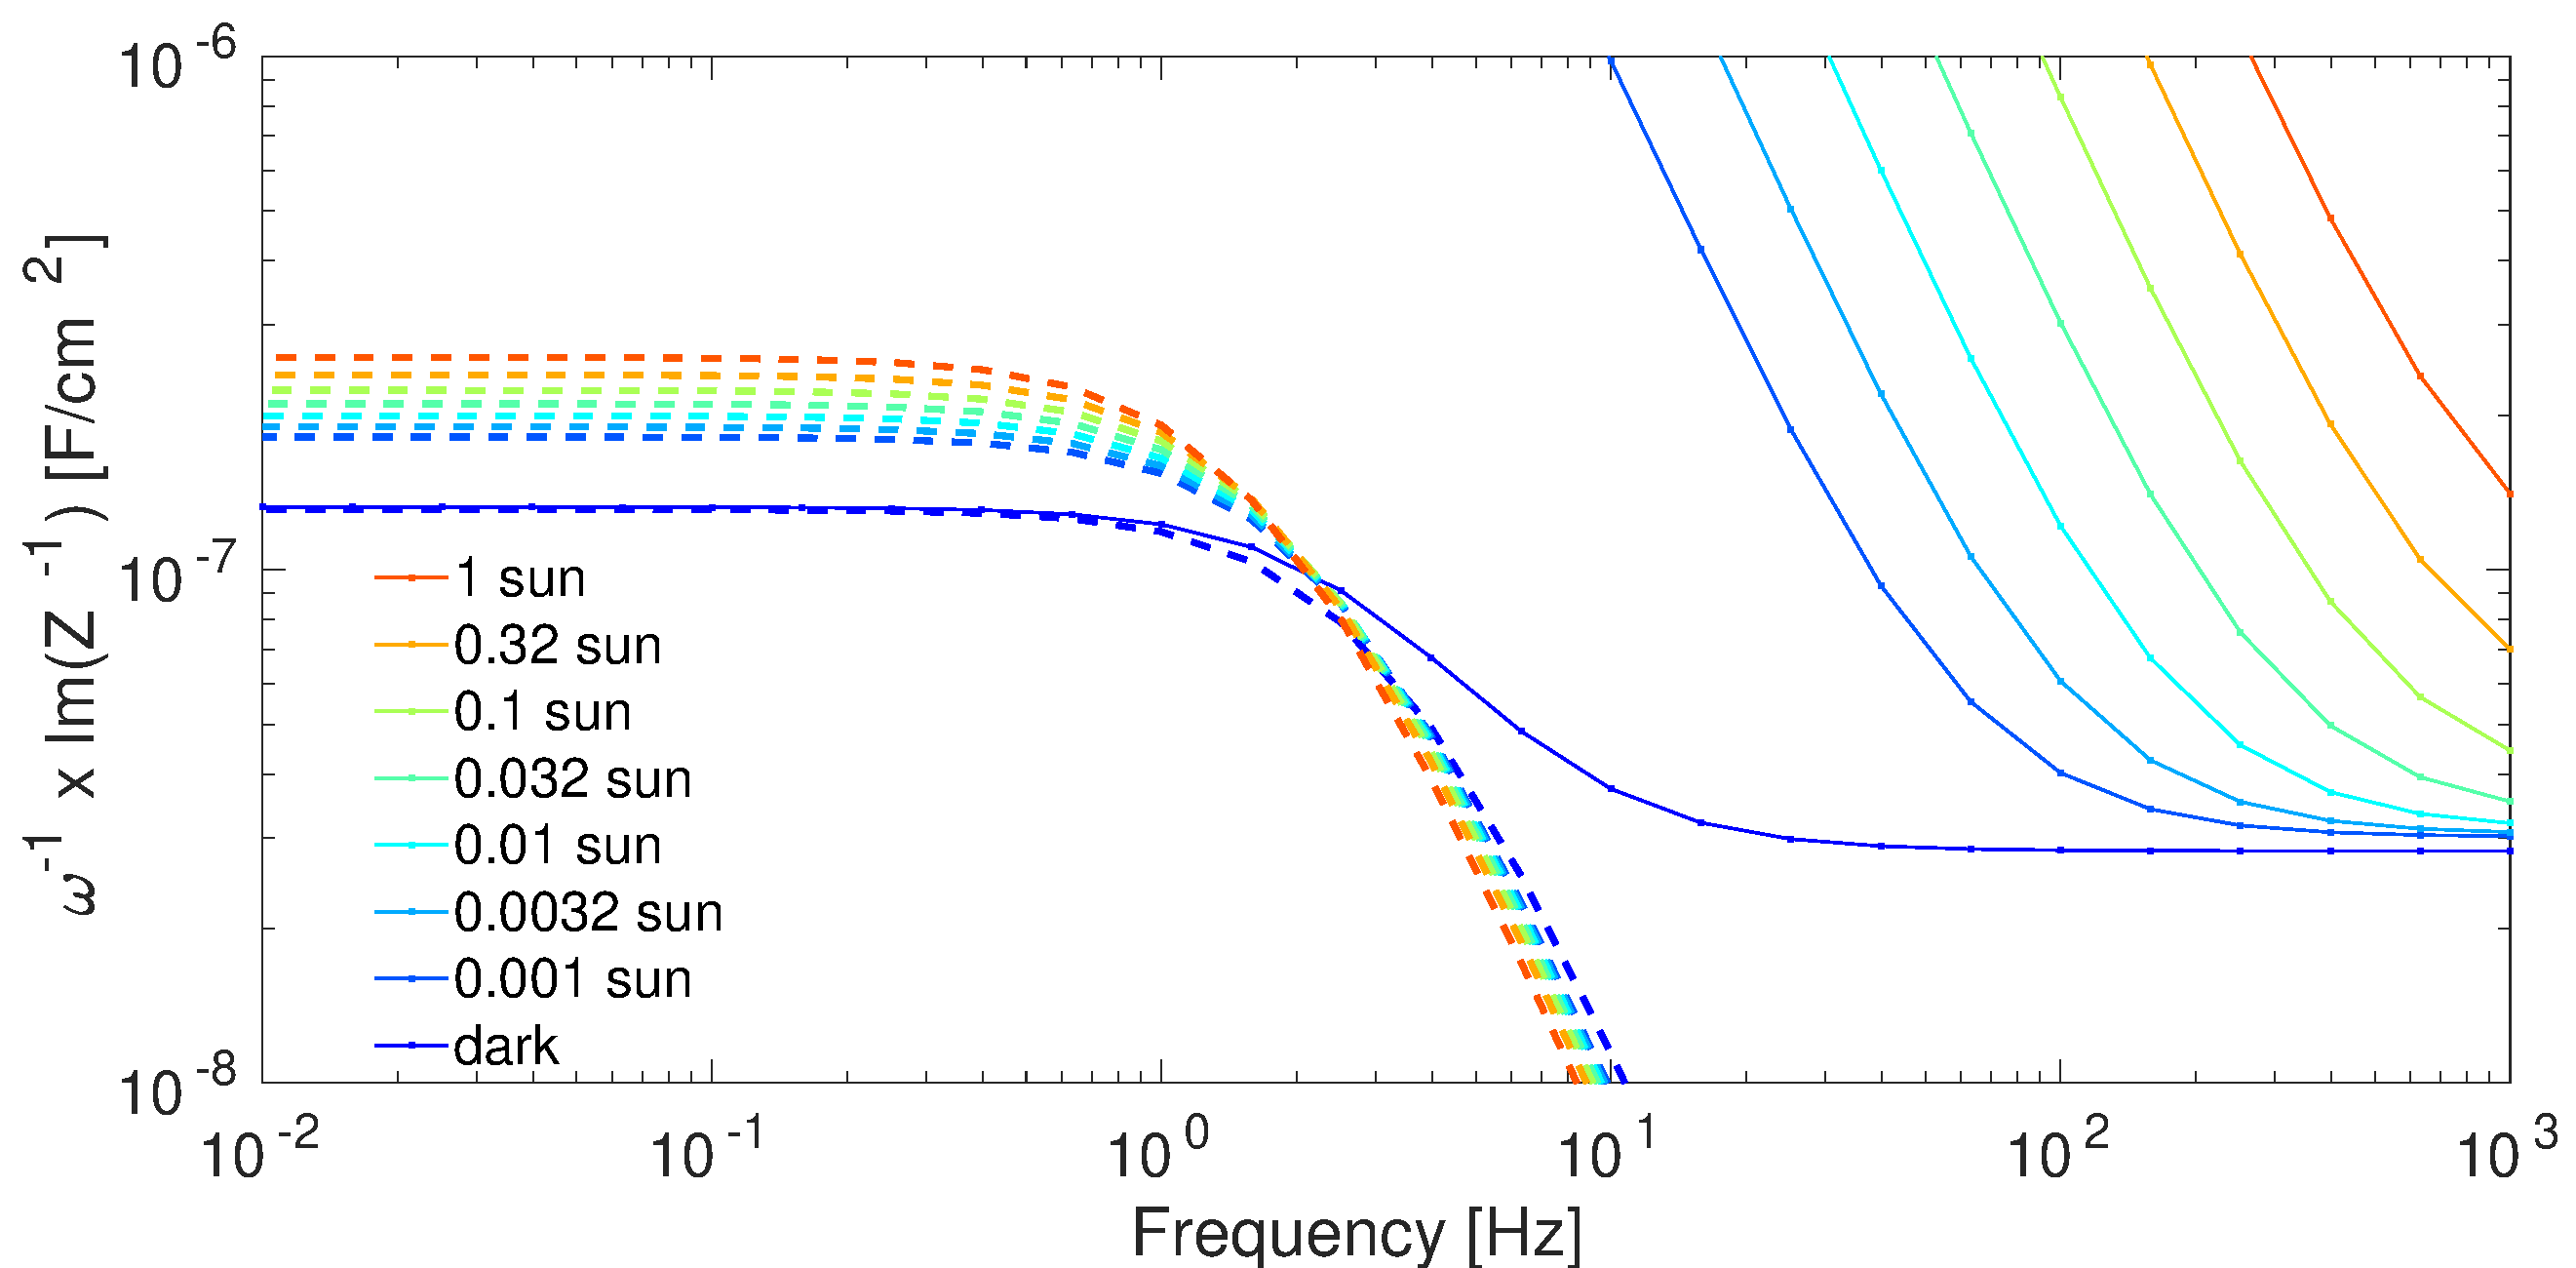
\includegraphics[width=1.05\textwidth]{dd_capacitance/ionic.pdf}
					\subcaption{Ionic displacement current capacitance}\label{fig:impedance-ionic-capacitance}
				\end{subfigure}

				\mycaption[Simulated apparent capacitance and phase spectra compared with capacitance due to ionic migration.]{
					In (\textbf{a}) the phase of the impedance (solid lines, it is the same as the oscillating current phase but with the opposite sign) is plotted and compared with the phase of the ionic current (dashed lines, changed of sign for easing the comparison).
					In (\textbf{b}) the apparent capacitance spectra (solid lines) is compared with the capacitance calculated from the out of phase ionic current (dashed lines).
				}\label{fig:impedance-ionic}
			}
		}
	\end{figure}

	%\begin{figure}
	%	\centering
	%	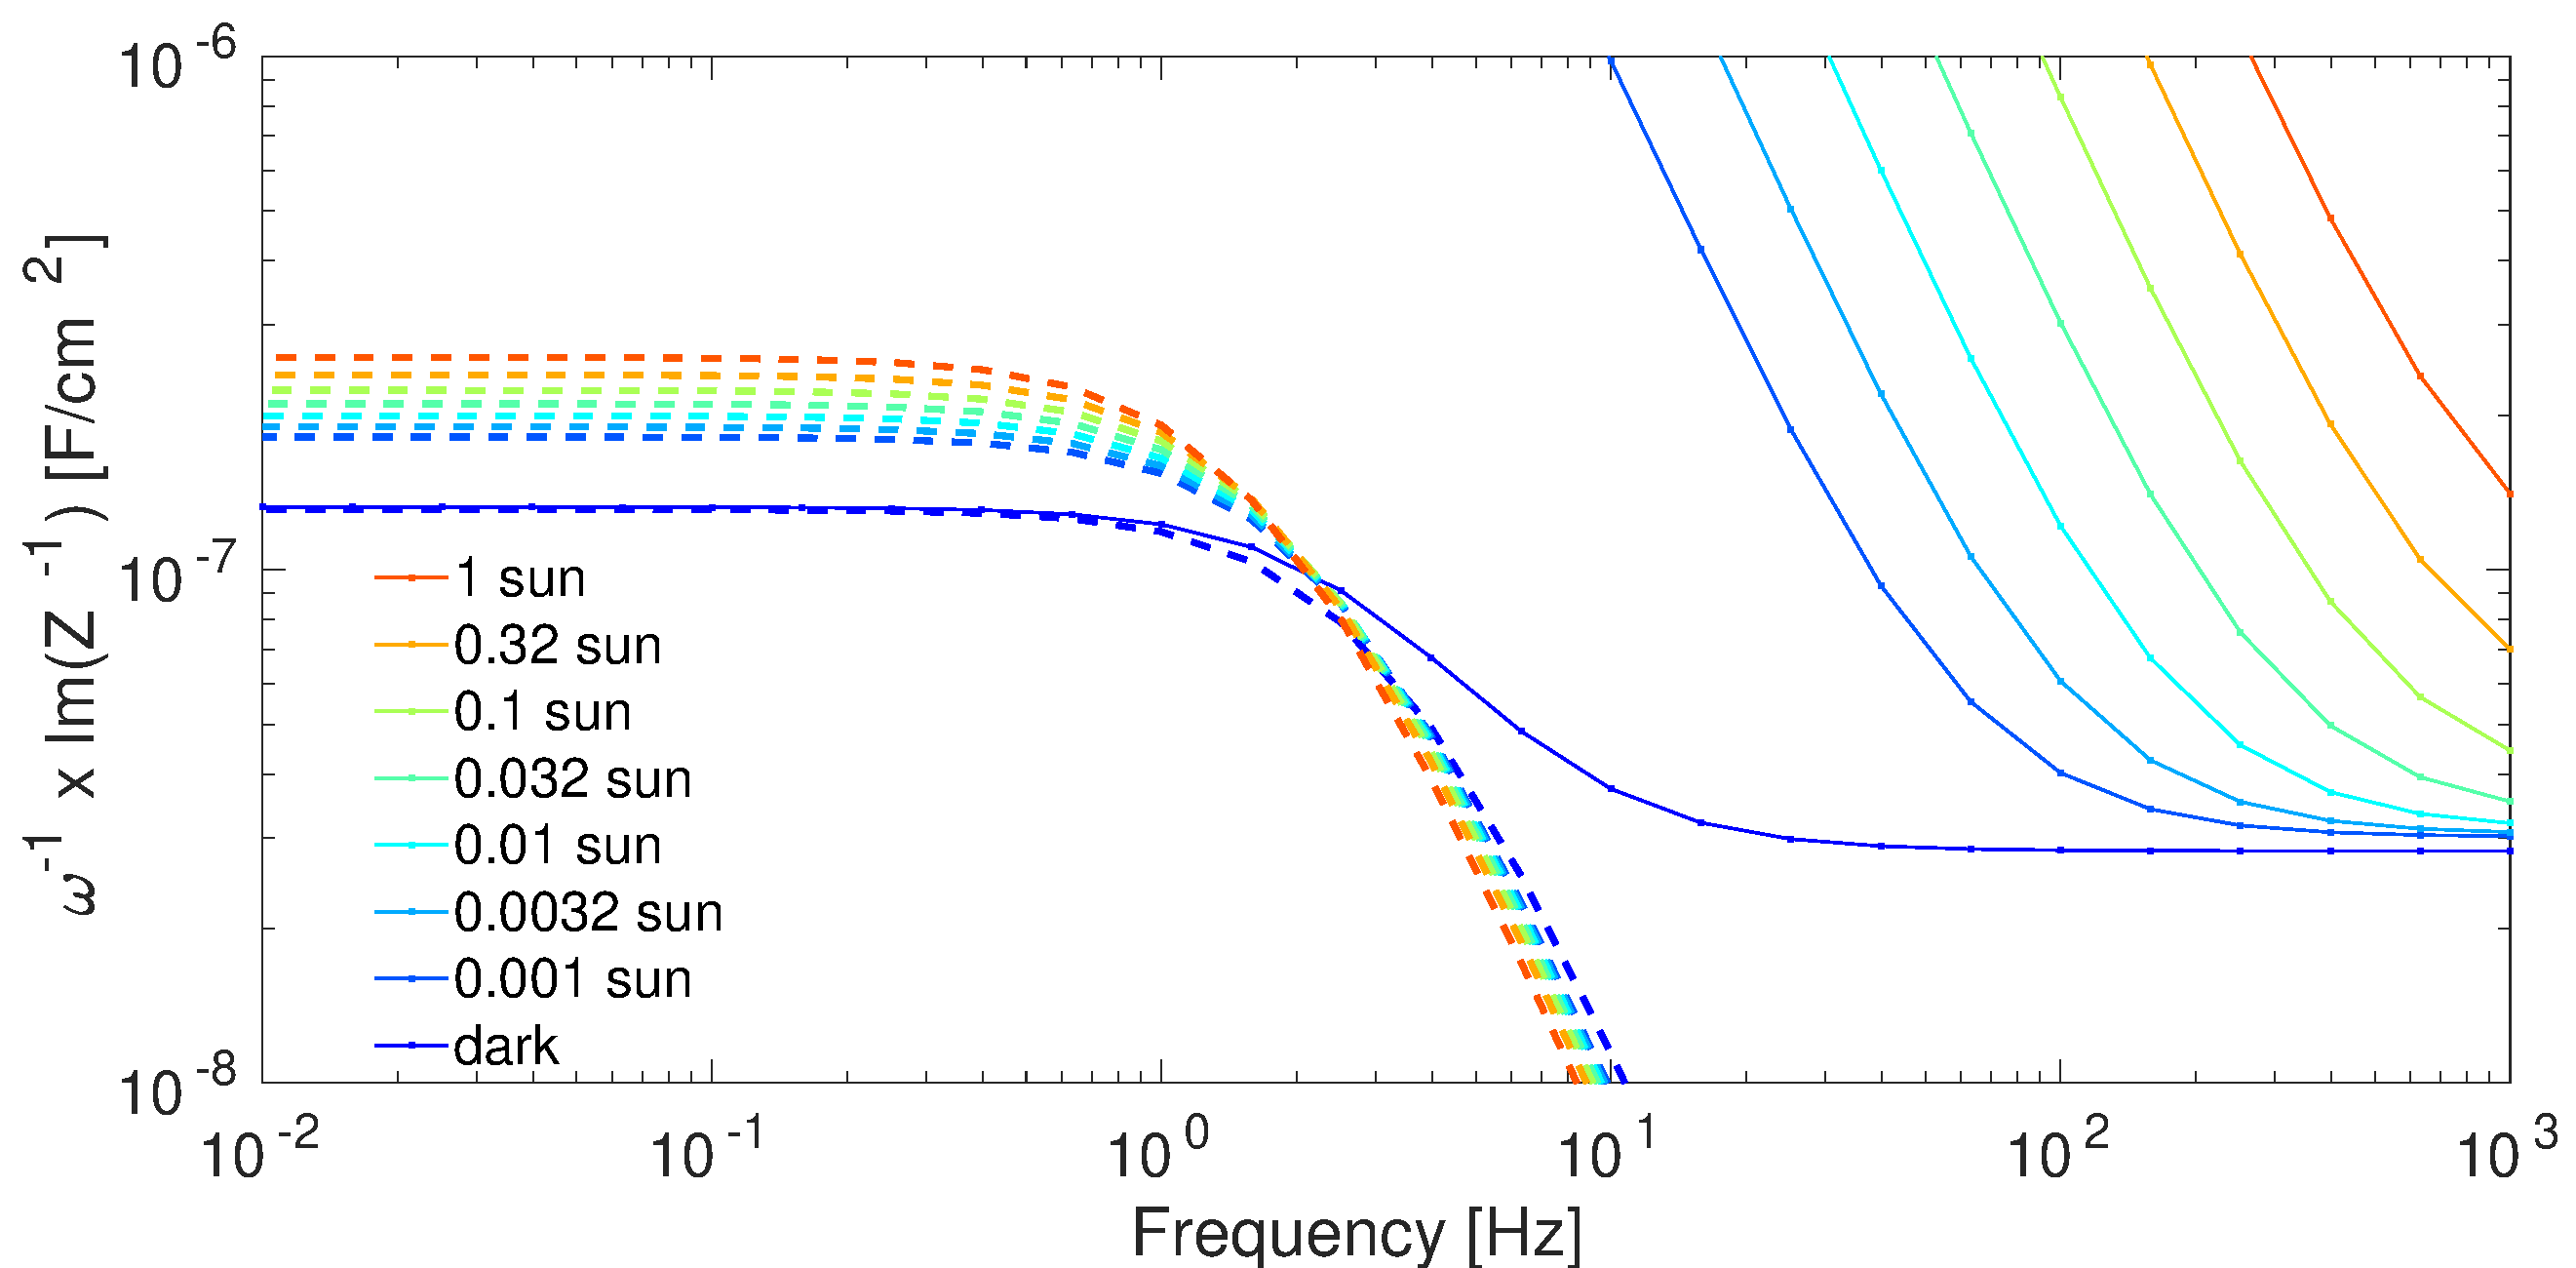
\includegraphics[width=1.1\textwidth]{dd_capacitance/ionic.pdf}
	%	\mycaption[Simulated ionic capacitance spectra of an illuminated perovskite solar cell.]{}\label{fig:impedance-ionic}
	%\end{figure}

	\paragraph{Dark case}
	An feature at frequencies \SI{< 100}{\Hz} is often observed in impedance of perovskite solar cells in dark \cite{Pockett2015,Juarez-Perez2014}.
	This feature has been interpreted as a ionic influence on the dark capacitance by \authoryear{Yang2015e}.


	\begin{figure}%impedance-recombination_nyquist
		\makebox[\textwidth][c]{
			\parbox{1.1\textwidth}{
				\centering
				\begin{subfigure}[t]{1.1\textwidth}
					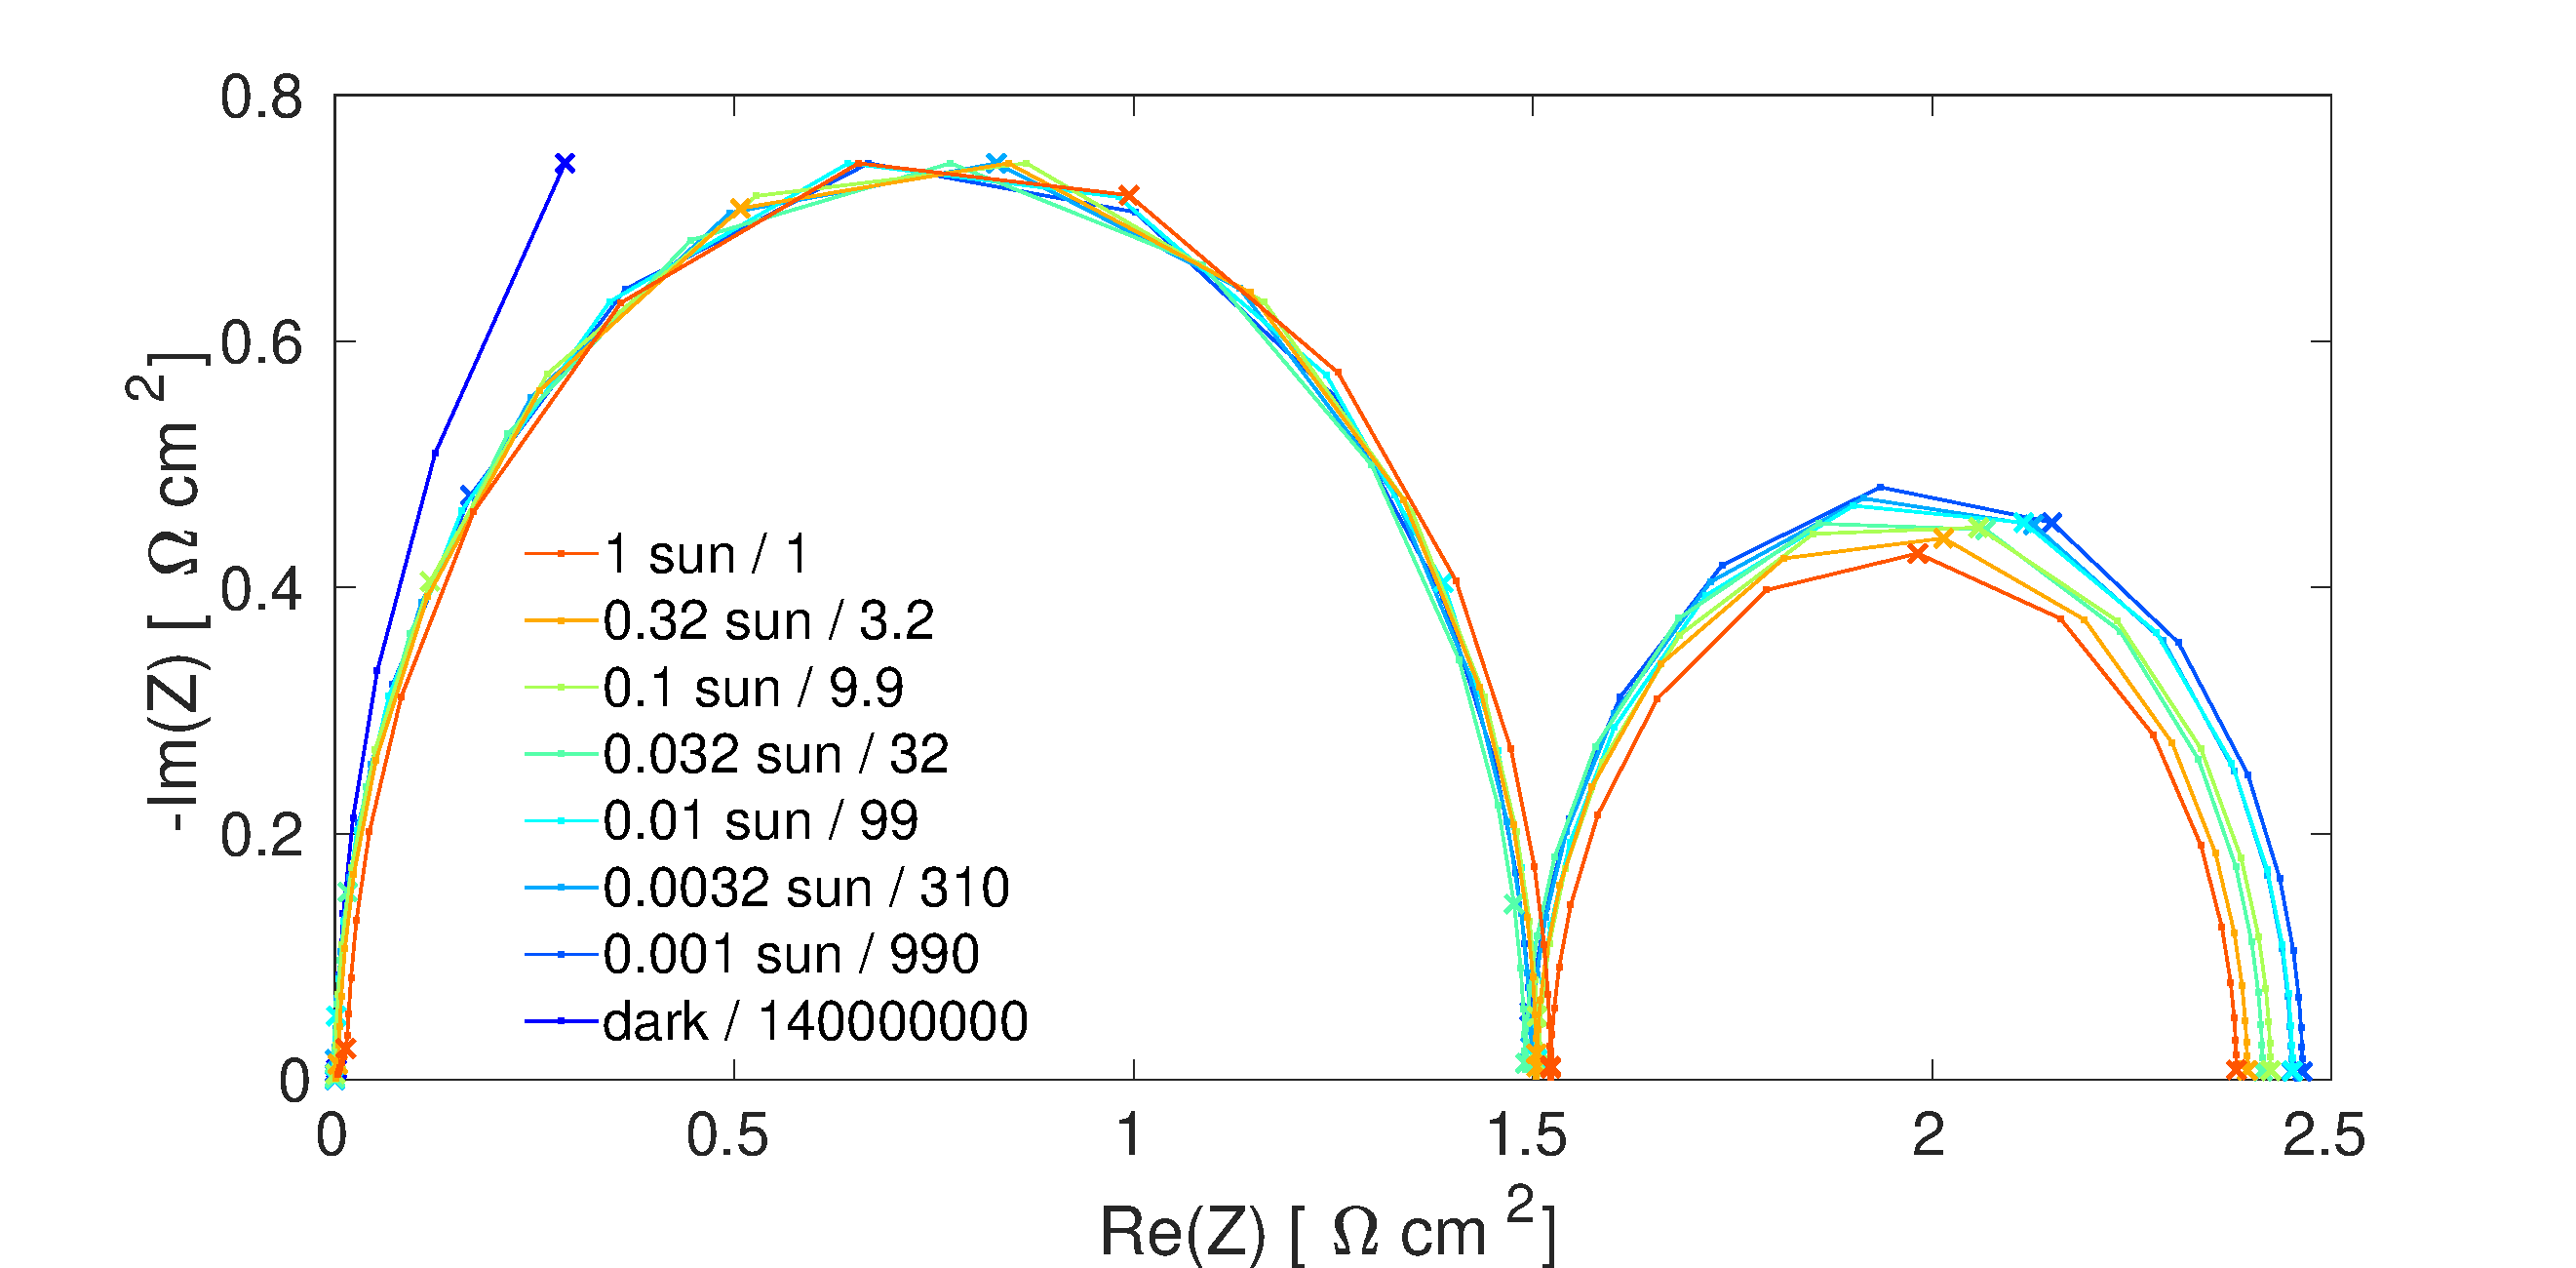
\includegraphics[width=1.05\textwidth]{dd_nyquist/nyquist_normalised.pdf}
					\subcaption{Nyquist plot}\label{fig:impedance-nyquist}
				\end{subfigure}
				\bigskip

				\begin{subfigure}[t]{1.1\textwidth}
					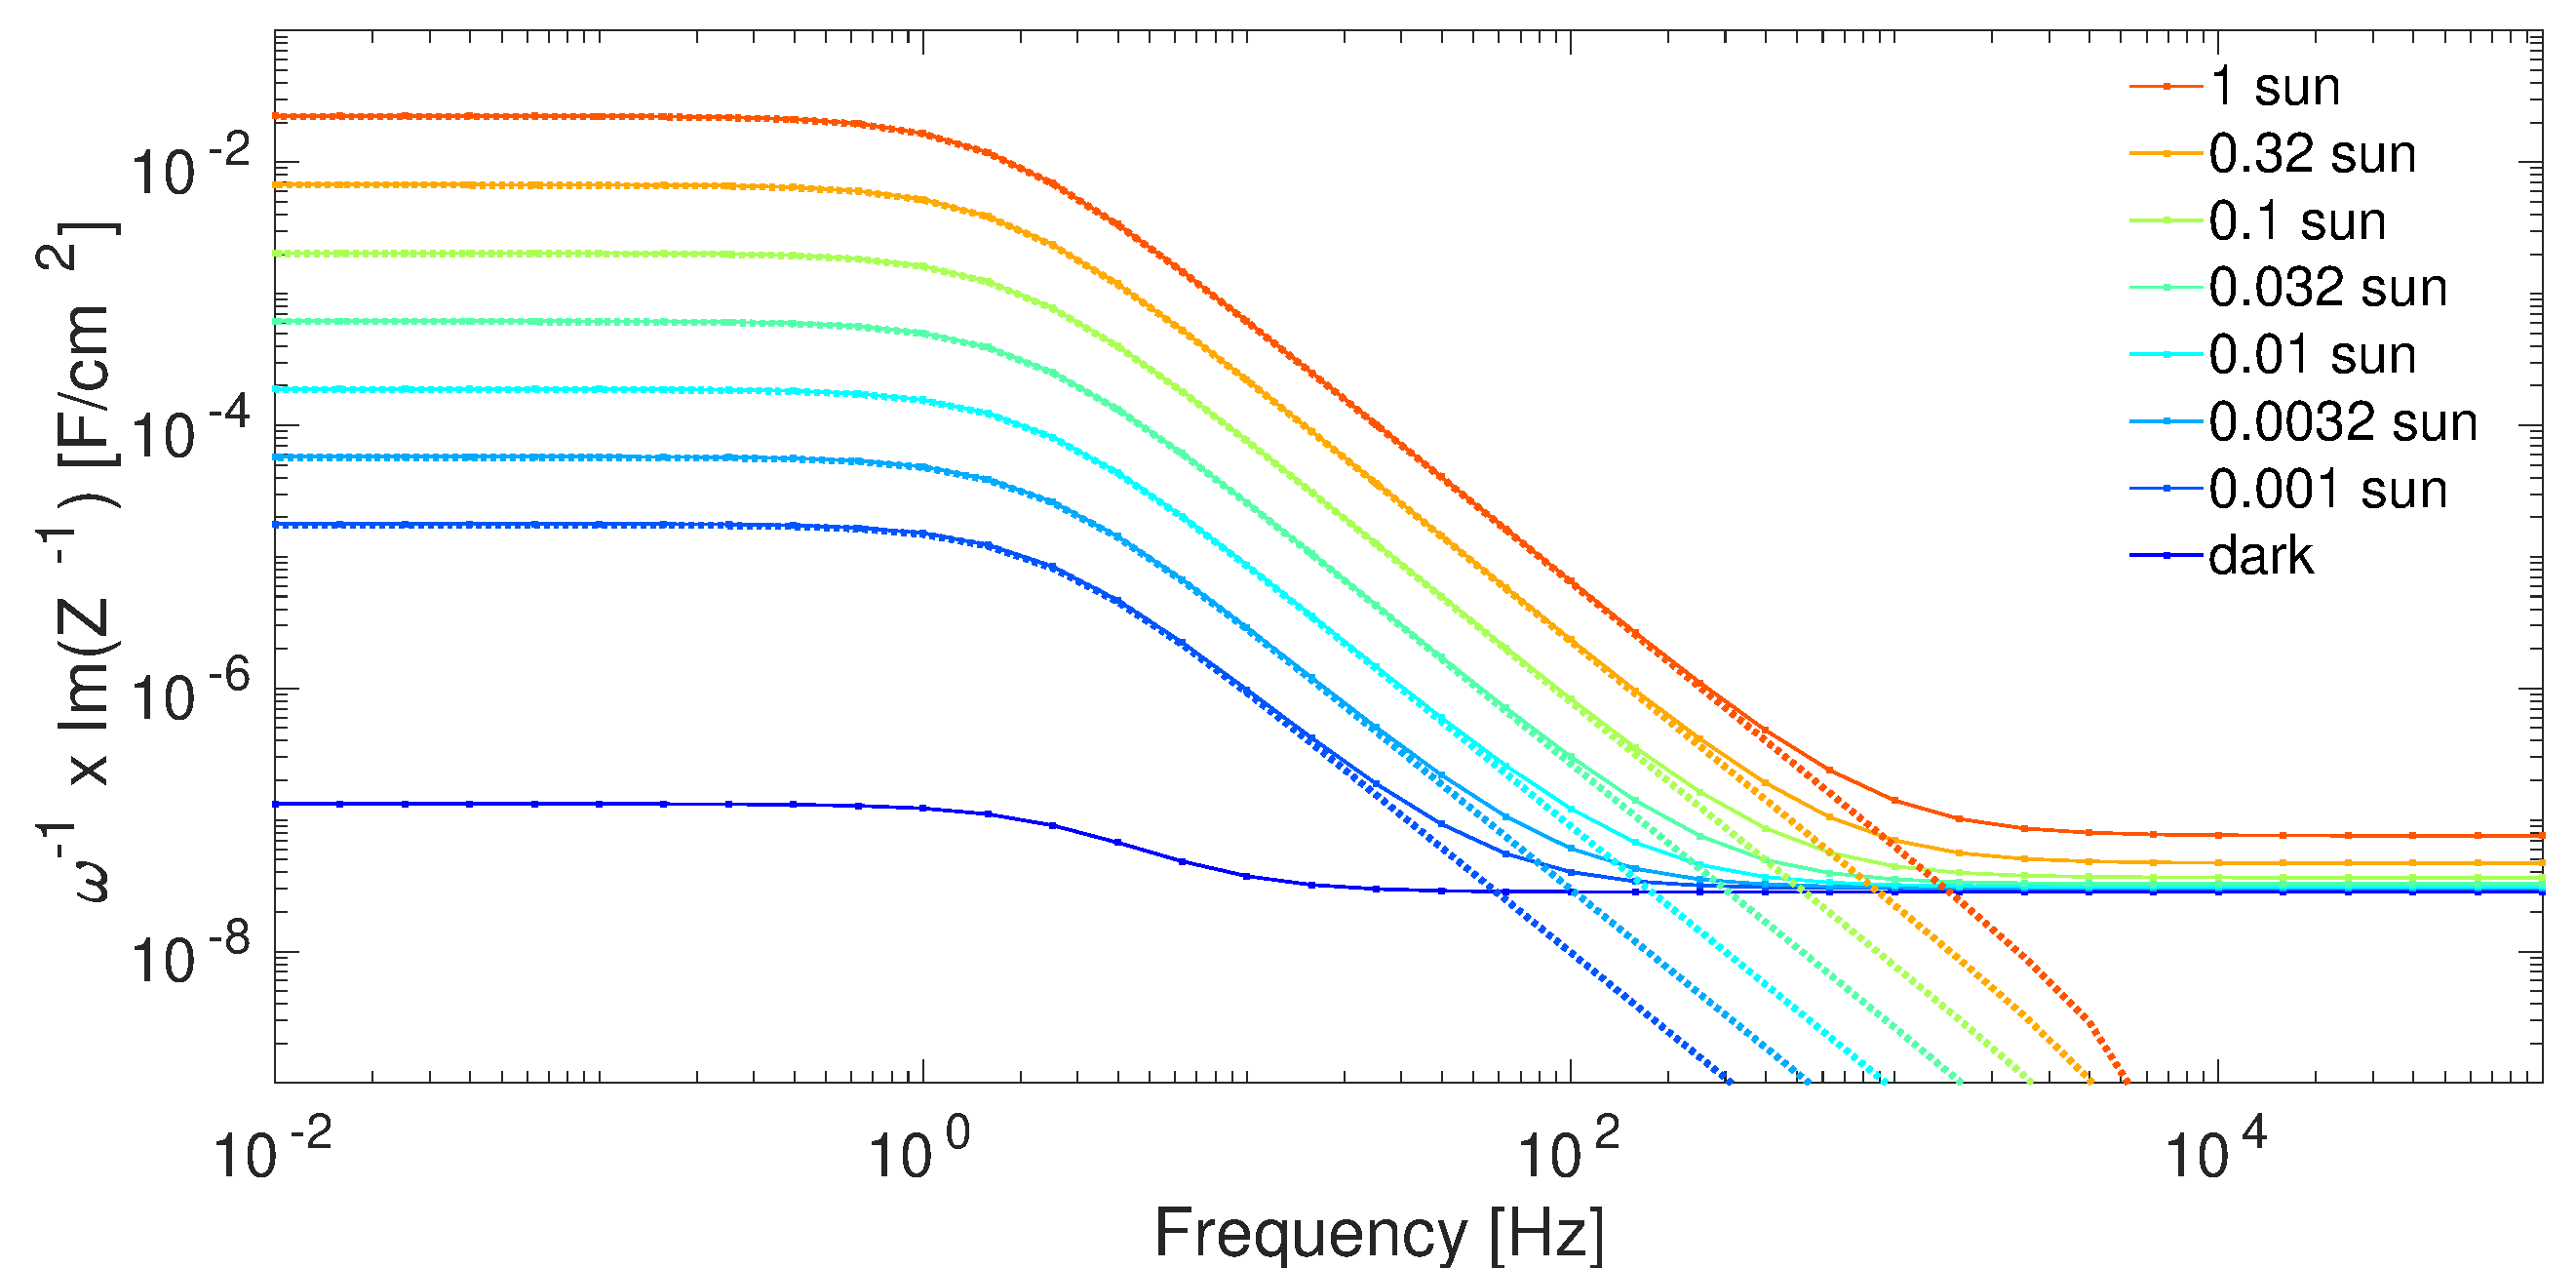
\includegraphics[width=1.05\textwidth]{dd_capacitance/recombination.pdf}
					\subcaption{Apparent capacitance from recombination current}\label{fig:impedance-recombination}
				\end{subfigure}

				\mycaption[Simulated apparent capacitance spectra and Nyquist plot compared with capacitance due to recombination current.]{
					In (\textbf{a}) the normalised Nyquist plot is reported, the normalisation factor is reported in the legend.
					The cross markers indicate the even frequency decades (\textsl{i.e.} from right to left \num{0.01}, \num{1}, \SI{100}{\Hz} \dots) so that the mid frequency minimum of 1~sun curve is around \SI{1000}{\Hz}.
					In (\textbf{b}) the apparent capacitance spectra (solid lines) is compared with the capacitance calculated from the out of phase recombination flux (dotted lines).
				}\label{fig:impedance-recombination_nyquist}
			}
		}
	\end{figure}



	\begin{figure}%diode_transistor
		\makebox[\textwidth][c]{
			\parbox{1.1\textwidth}{
				\centering
				\begin{subfigure}[t]{0.51\textwidth}
					\includegraphics[width=1\textwidth]{diode_transistor/CB-high_freq.pdf}
					\subcaption{Conduction band at high frequency}\label{fig:diode_transistor-band_diagram_hifreq}
				\end{subfigure}
				\qquad
				\begin{subfigure}[t]{0.51\textwidth}
					\includegraphics[width=1\textwidth]{diode_transistor/CB-low_freq.pdf}
					\subcaption{Conduction band at low frequency}\label{fig:diode_transistor-band_diagram_lowfreq}
				\end{subfigure}
				\bigskip

				\begin{subfigure}[t]{0.51\textwidth}\centering
					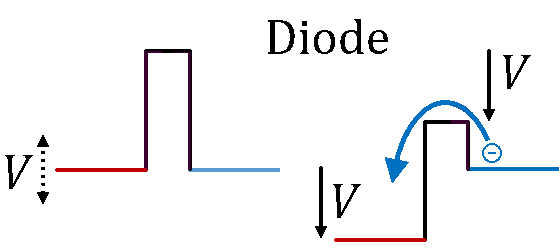
\includegraphics[width=0.7\textwidth]{diode_transistor/diode_scheme.png}
					\subcaption{Energy barrier in a diode}\label{fig:diode_transistor-diode_scheme}
				\end{subfigure}
				\qquad
				\begin{subfigure}[t]{0.51\textwidth}\centering
					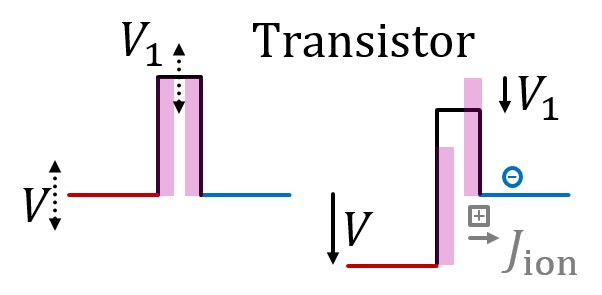
\includegraphics[width=0.8\textwidth]{diode_transistor/transistor_scheme.png}
					\subcaption{Energy barrier in a transistor}\label{fig:diode_transistor-transistor_scheme}
				\end{subfigure}
				\bigskip

				\begin{subfigure}[t]{0.51\textwidth}
					\includegraphics[width=1\textwidth]{diode_transistor/diode.png}
					\subcaption{Equivalent circuit with diode}\label{fig:diode_transistor-diode}
				\end{subfigure}
				\qquad
				\begin{subfigure}[t]{0.51\textwidth}
					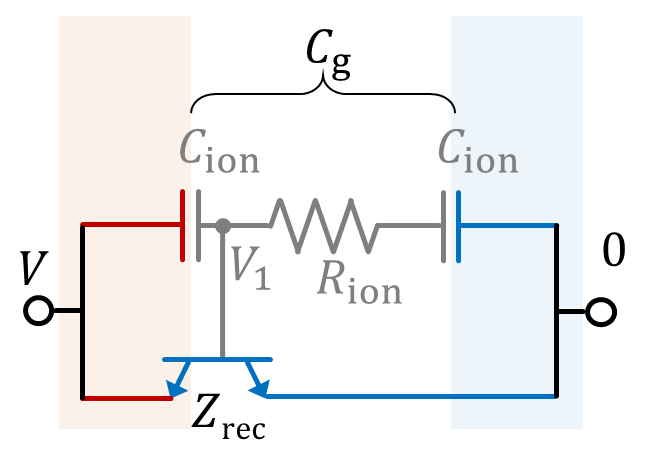
\includegraphics[width=0.9\textwidth]{diode_transistor/transistor.png}
					\subcaption{Equivalent circuit with transistor}\label{fig:diode_transistor-transistor}
				\end{subfigure}
				\mycaption[Band diagram, energy barriers, and circuit representation of a diode or a transistor.]{
					The conduction band (solid lines) and electron quasi\hyp{}Fermi level (dashed lines) of a \gls{htm} (left) perovskite (centre) \gls{etm} (right) solar cell is represented as varied by an oscillating voltage at mid and high frequencies in (\textbf{a}) and at low frequencies in (\textbf{b}).
					In (\textbf{c}) the energy barrier (black line) in a diode with applied voltage $V$ is represented.
					In (\textbf{d}) the energy barrier in a transistor is represented, with contributions from the applied voltage $V$ and an external voltage $V_1$.
					Pink rectangles indicating the barrier for the non-biassed case are added as graphical reference.
					In (\textbf{e}) a classical circuit including the ionic capacitance and the Schottky junction diode is represented.
					In (\textbf{f}) the influence of ionic accumulation on the interfacial diode is made explicit by the inclusion of a transistor where the potential in ionic branch acts as a gate.
				}\label{fig:diode_transistor}
			}
		}
	\end{figure}


	\paragraph{Illuminated or biassed case}
Juarez-Perez2014


	\paragraph{Loops in the positive semi-plane and large perturbations}\label{impedance-large_perturbations}
		In \authoryear{Moia2019} we showed that the failure in stabilizing the device to the measurement conditions (temperature, background voltage, illumination) results in loops in the Nyquist plot positive semi-plane.
		Additionally, a large perturbation measurement, which is a wide sinusoidal voltage oscillation amplitude in impedance measurements, can cause a non-sinusoidal current output.
		This is not a problem for the measurement itself, as the lock-in amplifiers are perfectly able to extract the amplitude and the phase of the signal first harmonic, ignoring the higher harmonics caused by the too large perturbation.
		This observation comes merely from simulations, no experimental confirmation is available yet.
		%But artefacts could arise and cause misinterpretations.

		\begin{figure}%impedance-200mV
			\makebox[\textwidth][c]{
				\parbox{1.1\textwidth}{
					\centering
					\begin{subfigure}[t]{1.1\textwidth}
						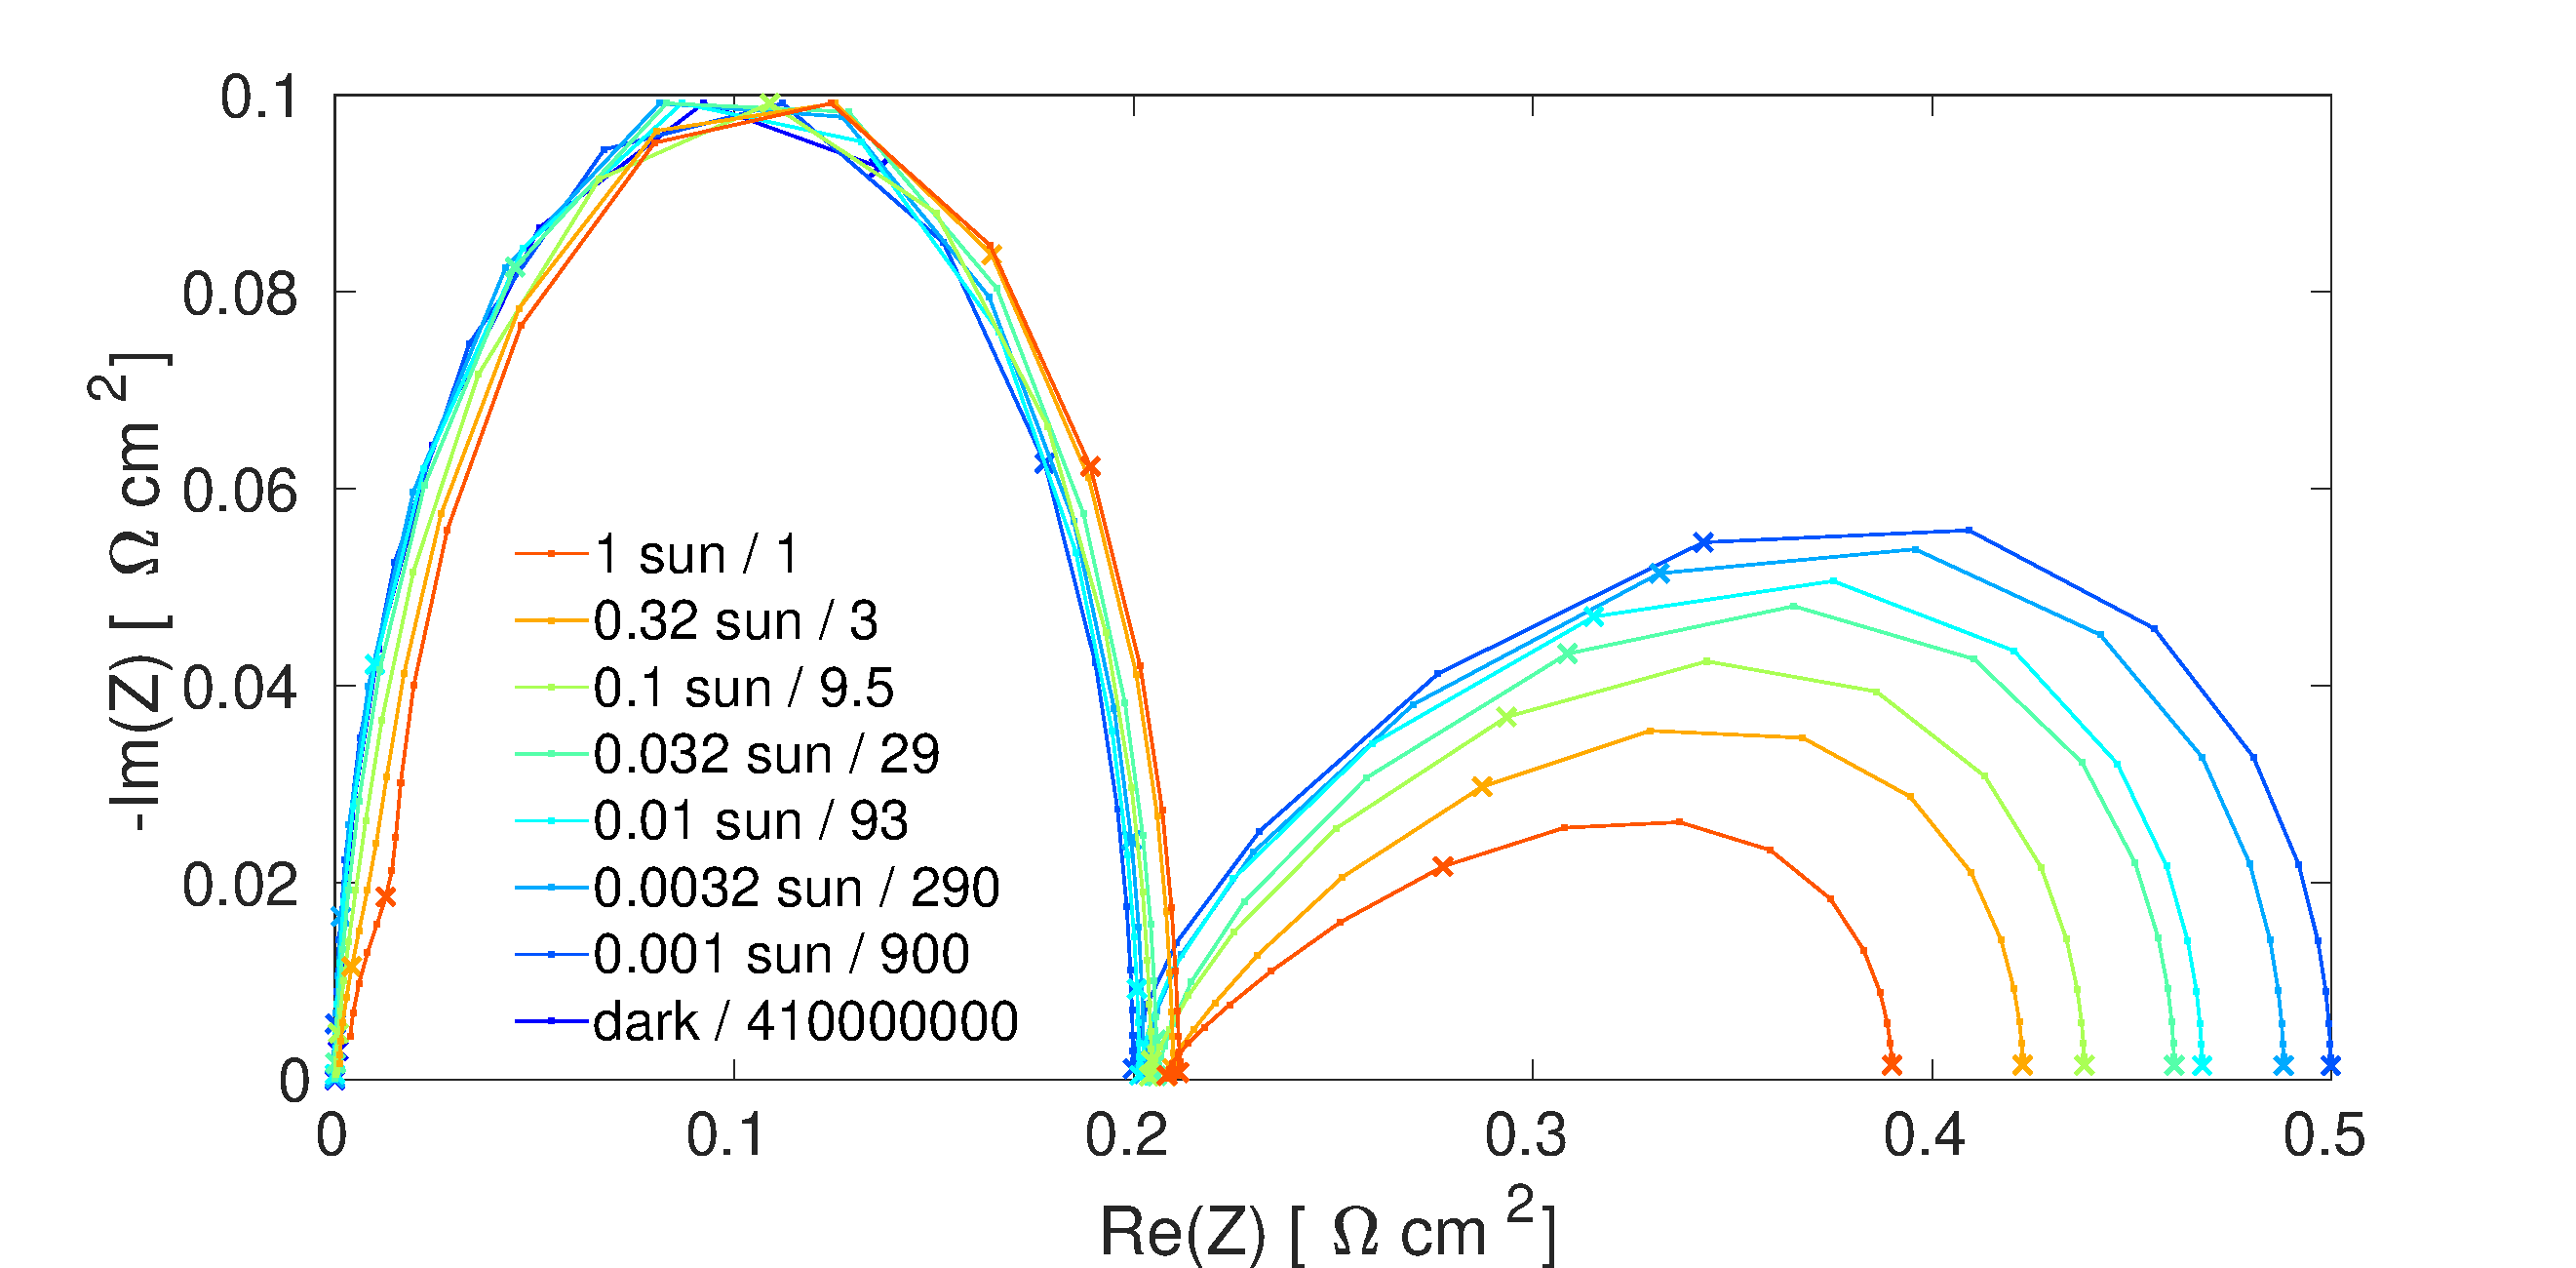
\includegraphics[width=1.05\textwidth]{dd_nyquist/nyquist_200mV_normalised.pdf}
						\subcaption{Nyquist plot with large perturbations}\label{fig:impedance-200mV_nyquist}
					\end{subfigure}
					\bigskip

					\begin{subfigure}[t]{1.1\textwidth}
						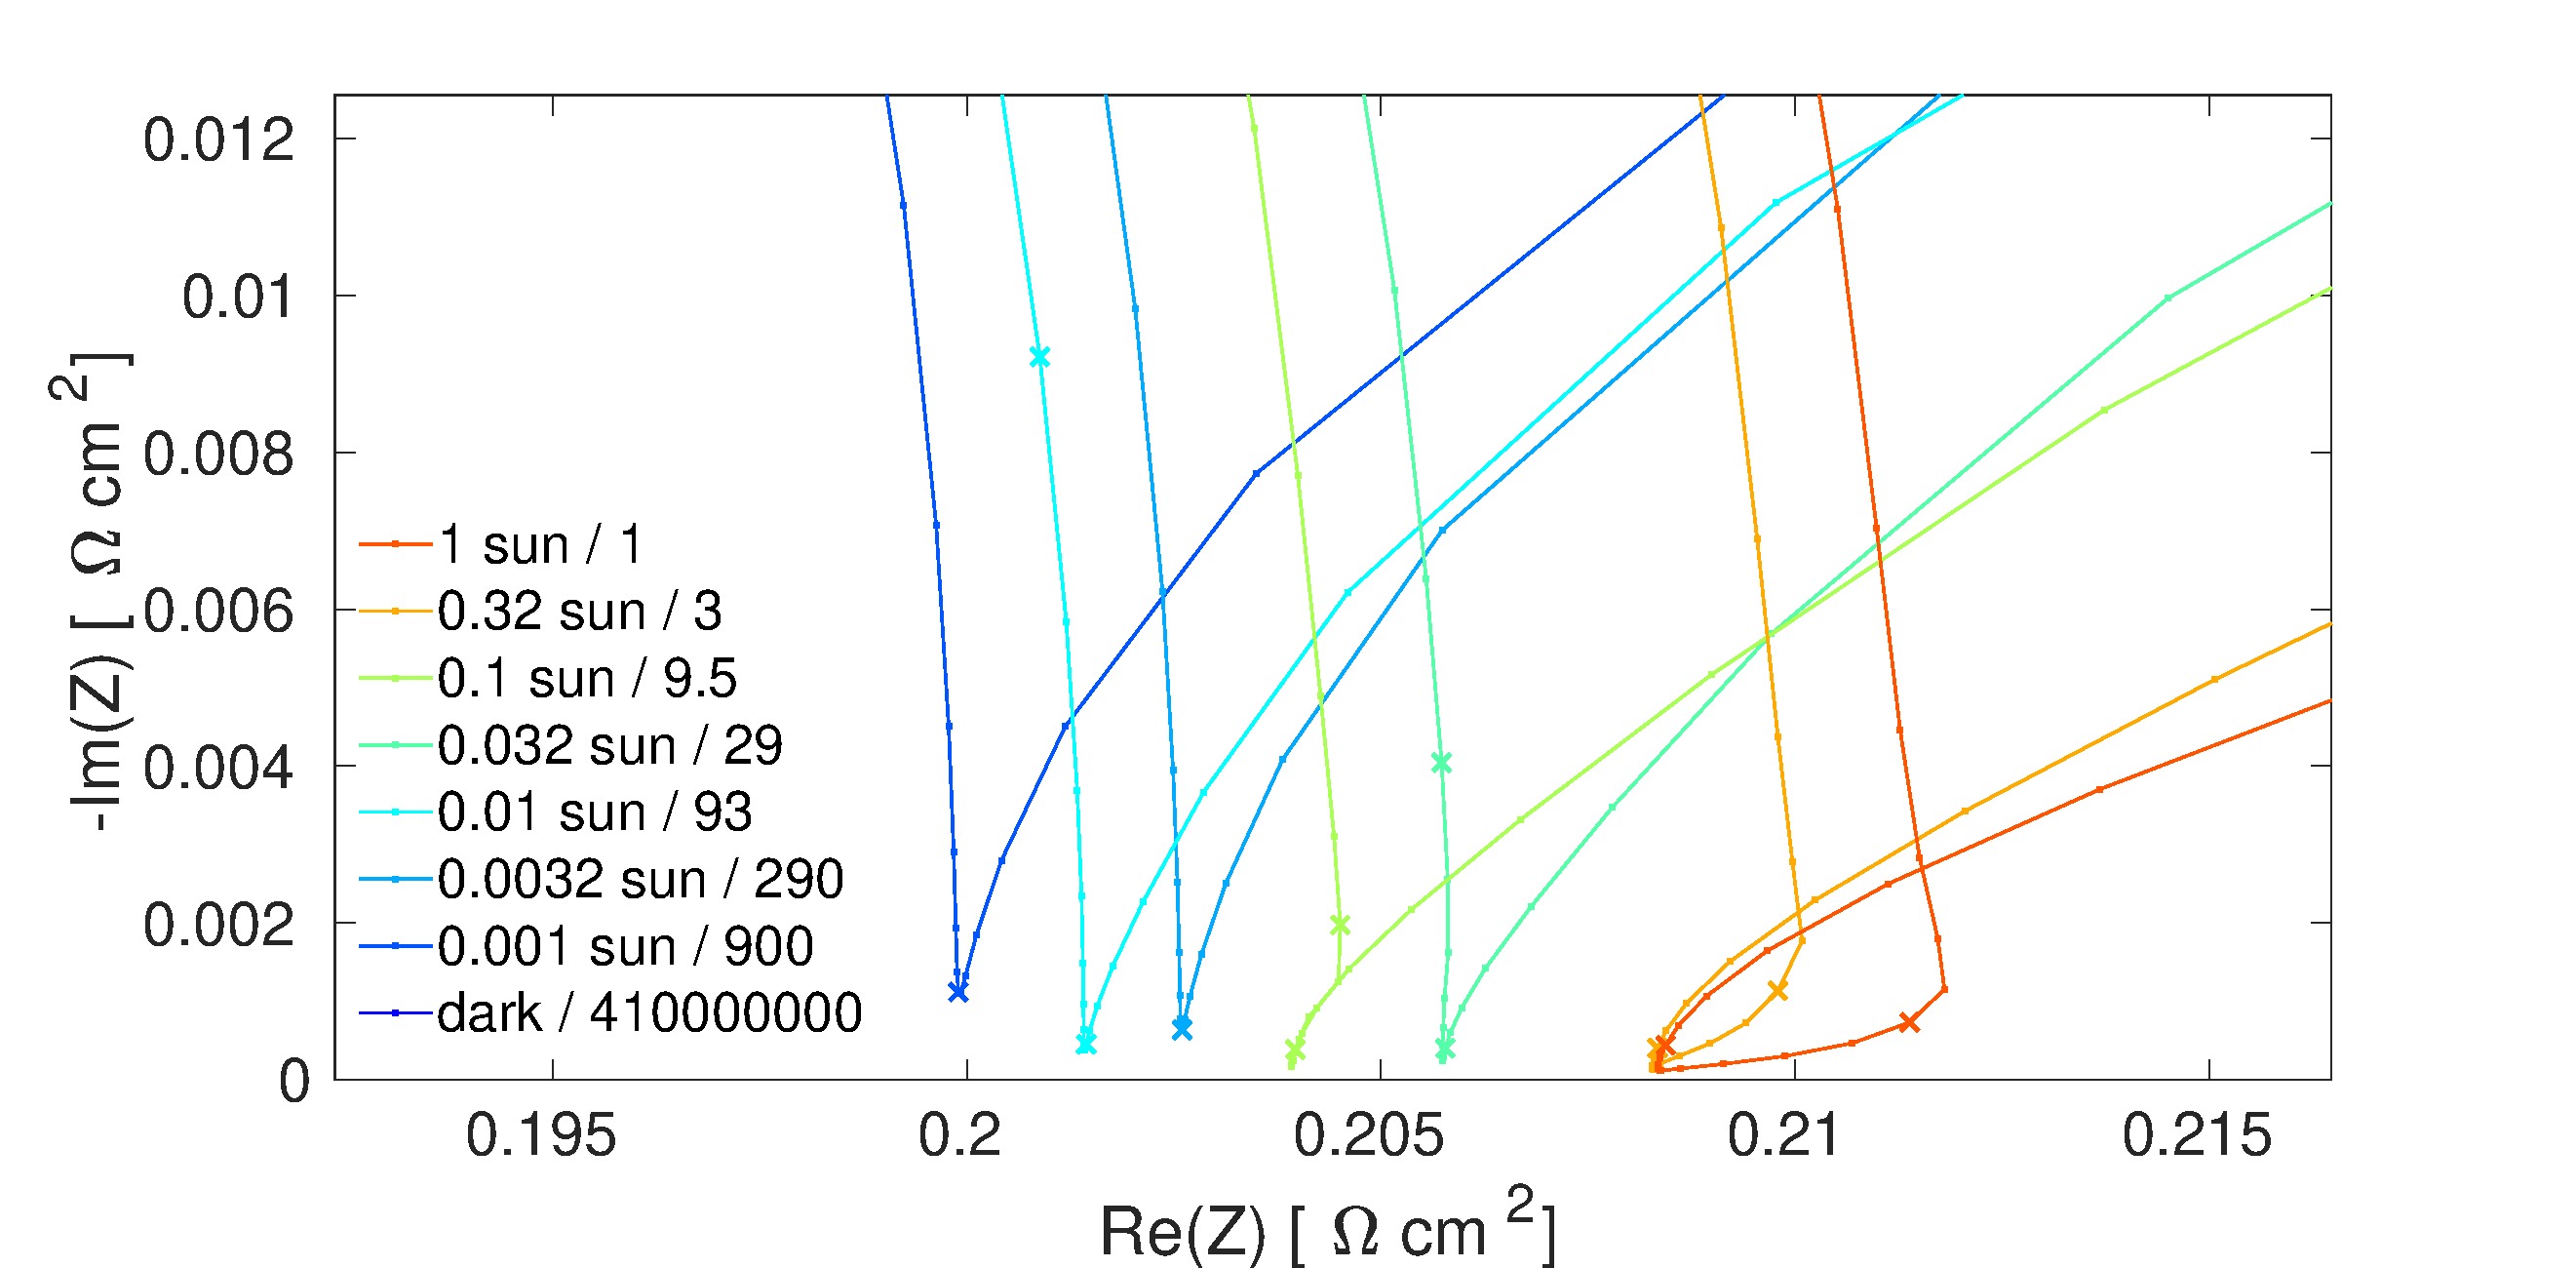
\includegraphics[width=1.05\textwidth]{dd_nyquist/nyquist_200mV_normalised_zoom.pdf}
						\subcaption{Zoom into mid frequency region}\label{fig:impedance-200mV_nyquist-zoom}
					\end{subfigure}
					\mycaption[Simulated Nyquist plot for large perturbations simulation.]{
						In (\textbf{a}) the normalised Nyquist plot of a simulation with \SI{200}{\mV} wide oscillating applied voltage is represented.
						Normalisation factor is indicated in the legend.
						In (\textbf{b}) zoom at mid frequencies region of the same Nyquist plot, where loops can be observed in the high intensity curves.
					}\label{fig:impedance-200mV}
				}
			}
		\end{figure}


		\mysection[Comparison of simulation and experiment]{Comparison of simulated and experimental impedance spectra}
		


		\begin{figure}%experimental
			\makebox[\textwidth][c]{
				\parbox{1.1\textwidth}{
					\centering
					\begin{subfigure}[t]{0.51\textwidth}
						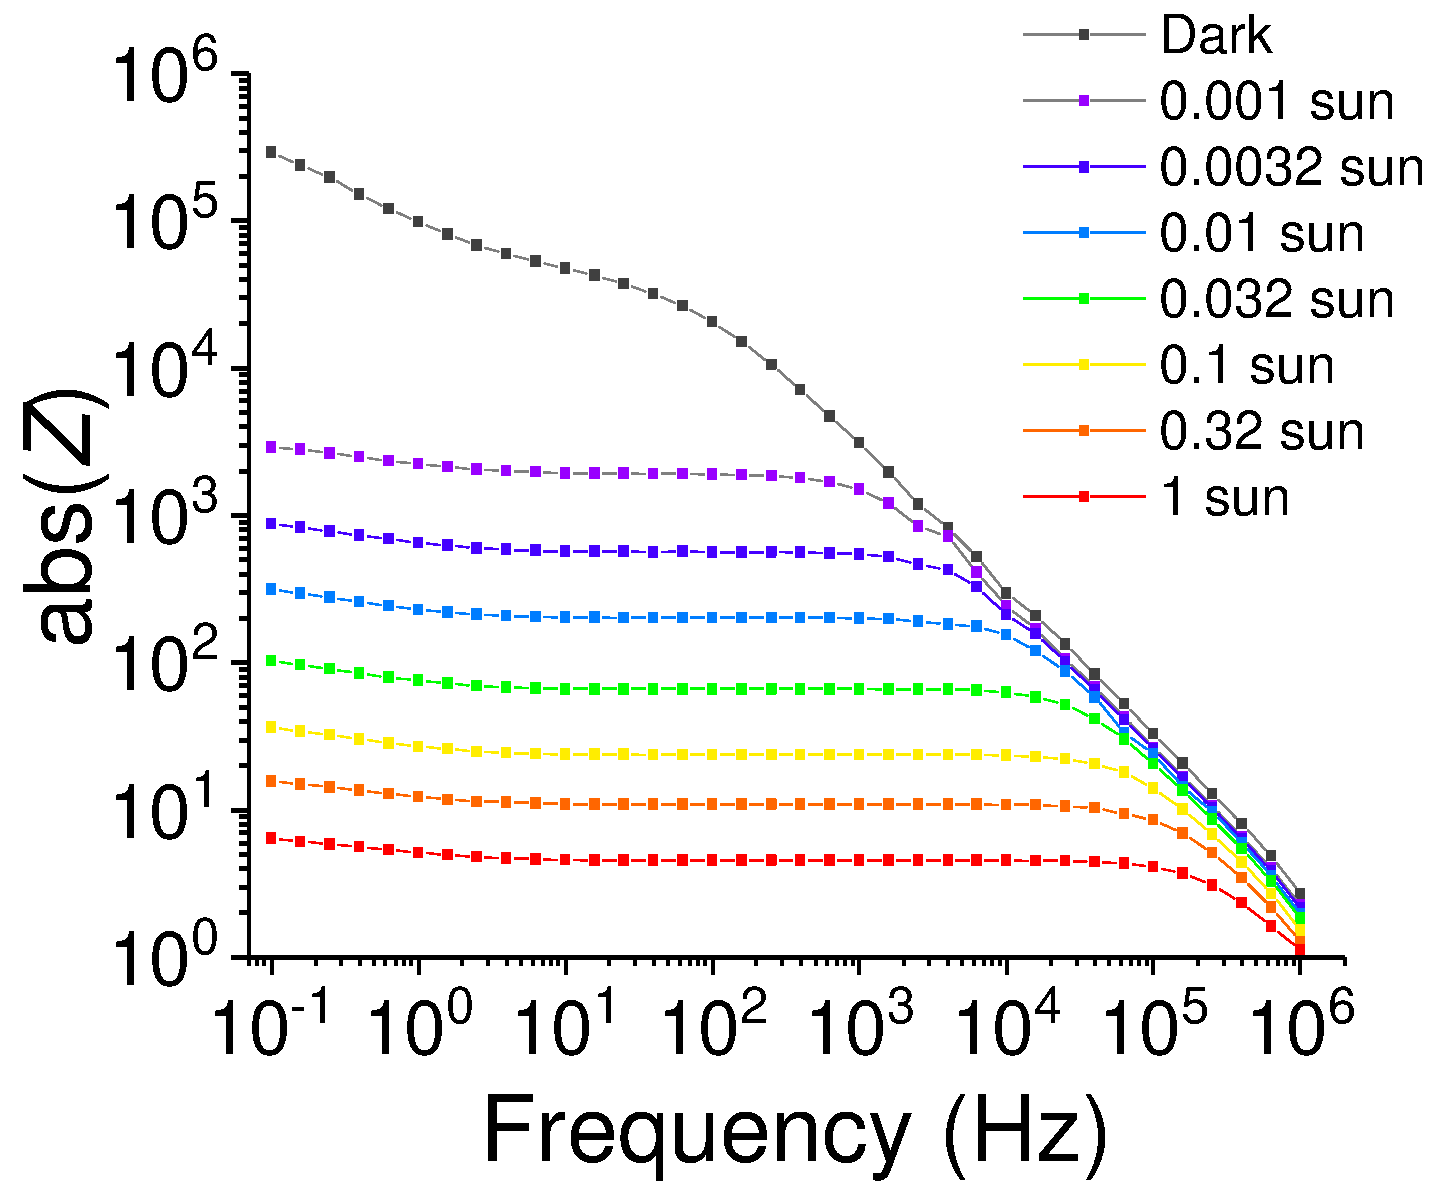
\includegraphics[width=1\textwidth]{experimental/Zabs-experimental.pdf}
						\subcaption{Impedance module}\label{fig:experimental-Zabs}
					\end{subfigure}
					\qquad
					\begin{subfigure}[t]{0.51\textwidth}
						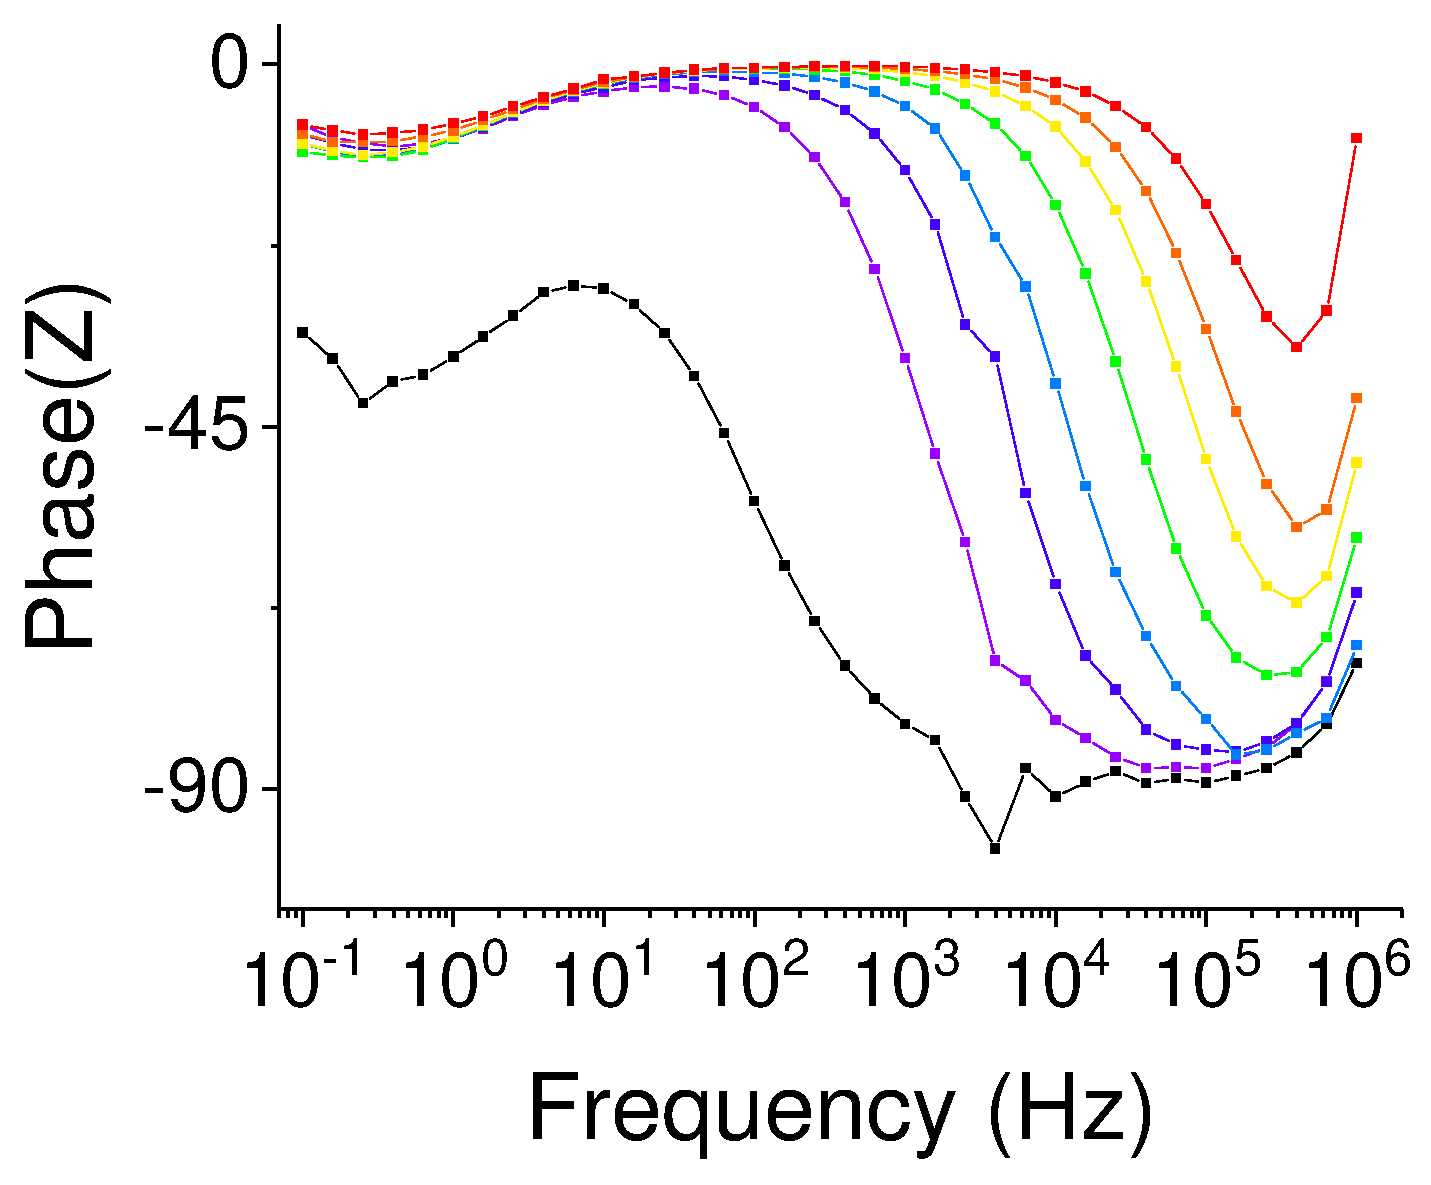
\includegraphics[width=1\textwidth]{experimental/phase-experimental.pdf}
						\subcaption{Impedance phase}\label{fig:experimental-phase}
					\end{subfigure}
					\bigskip

					\begin{subfigure}[t]{0.81\textwidth}
						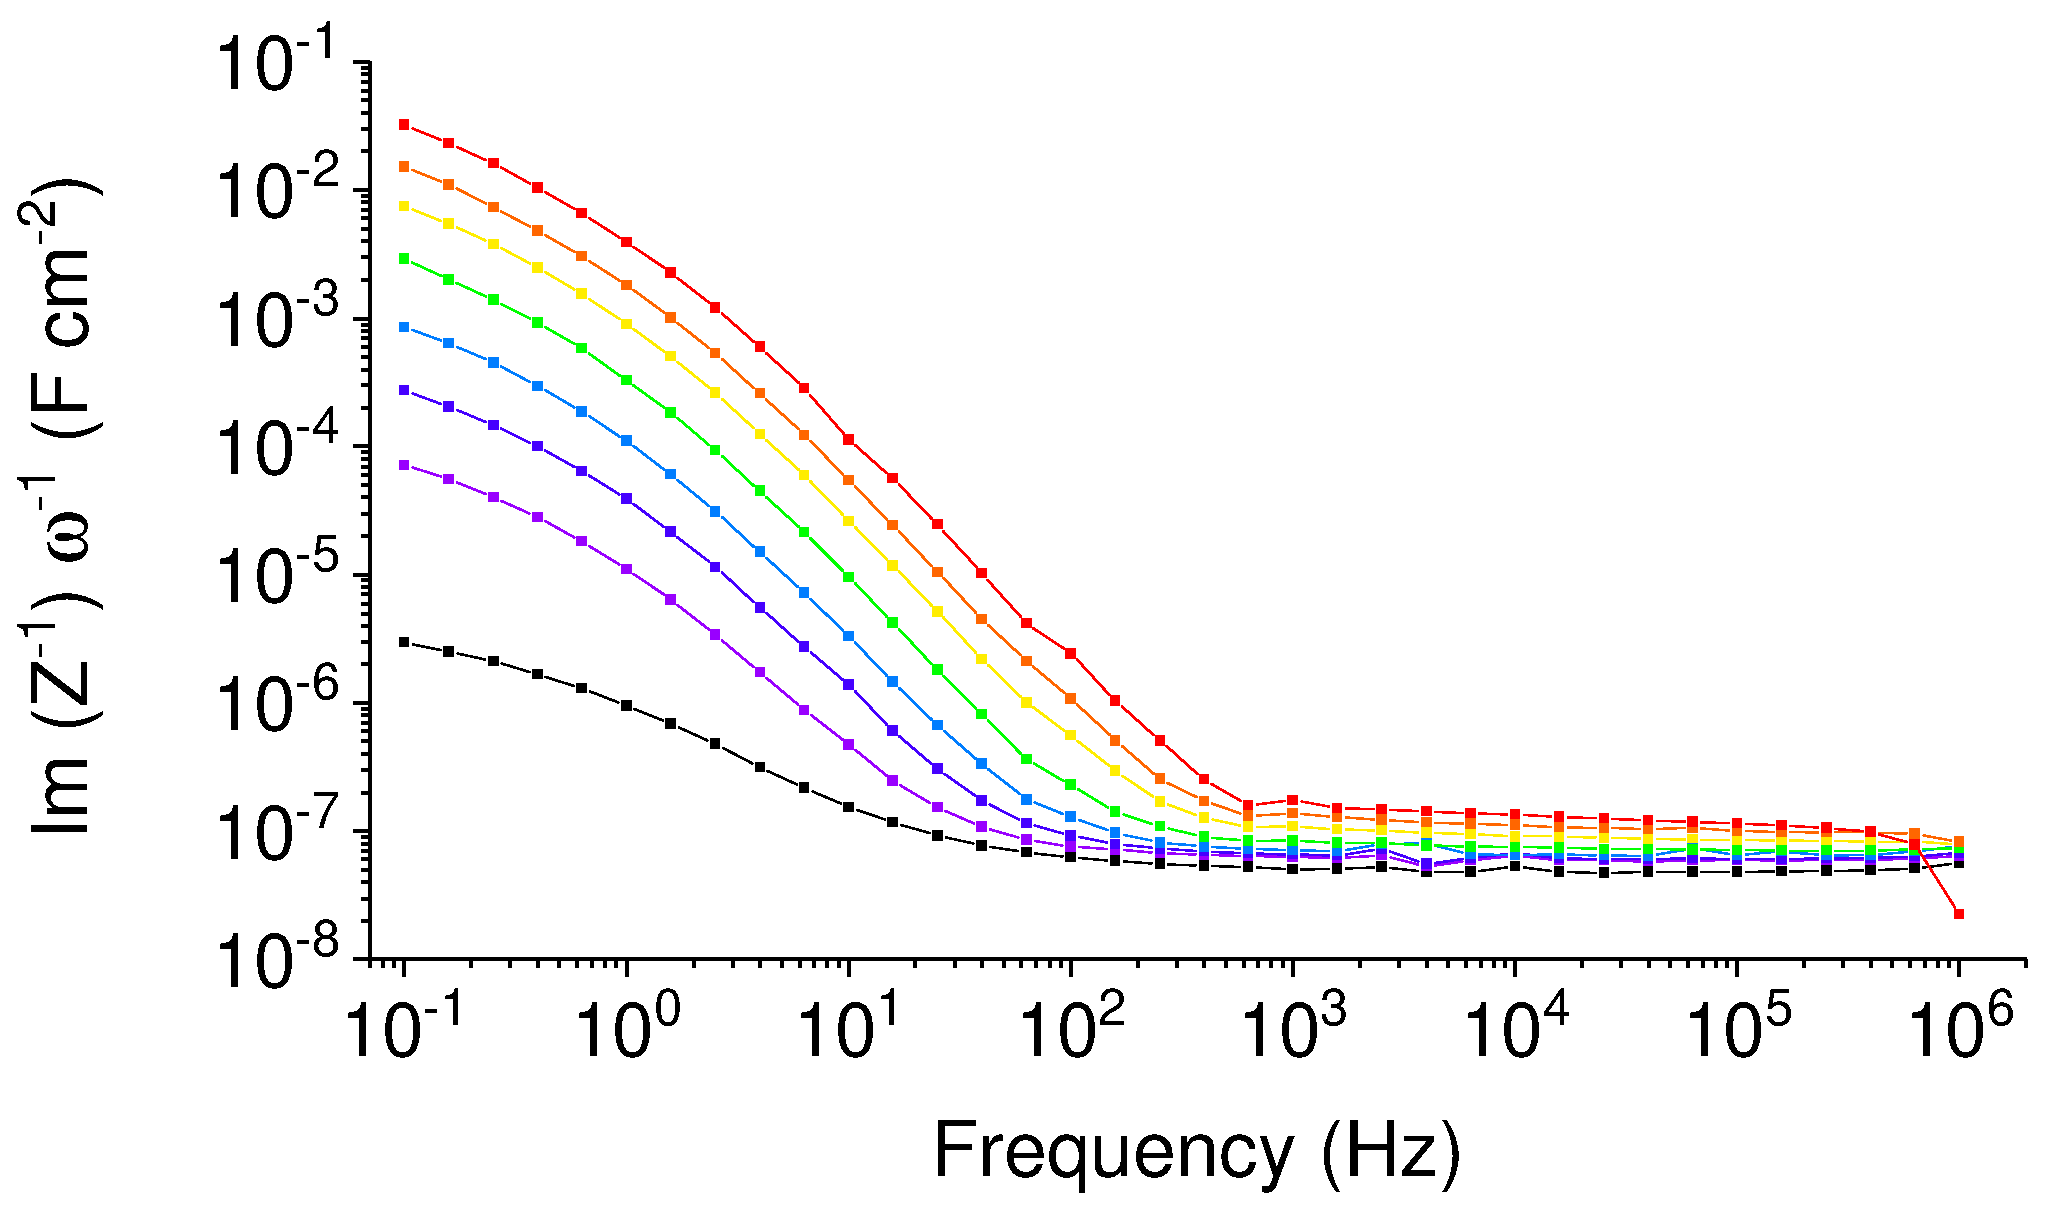
\includegraphics[width=1\textwidth]{experimental/cap-experimental.pdf}
						\subcaption{Apparent capacitance}\label{fig:experimental-cap}
					\end{subfigure}

					\mycaption[Experimental data from impedance spectroscopy of an illuminated perovskite solar cell at open circuit conditions.]{
						In (\textbf{a}) the absolute value of the experimental impedance is reported.
						In (\textbf{b}) the phase of the experimental impedance is reported, it can be compared with simulated data in \cref{fig:impedance-ionic-phase}.
						In (\textbf{c}) the experimental apparent capacitance is reported, it can be compared with simulated data in \cref{fig:impedance-capacitance}.
					}\label{fig:experimental}
				}
			}
		\end{figure}

		\paragraph{Lack of low frequency plateau}
		At low frequency we observe 
		
		%\paragraph{Larger ionic capacitance}

		\paragraph{Short circuit}
		Both the simulation at open circuit with illumination or at dark with applied background voltage bias matches quite nicely the experimental data.
		On the contrary, the simulation at short circuit with illumination showed a low frequency apparent capacitance increase of just 30 times from dark to 1~sun, while experimentally a giant capacitance is also observed.
		This discrepancy is left unexplained, a closer look is needed in order to understand which physical phenomena is not implemented in the model or, more simply, which variable is far from the realistic value.


\section{Implementation of impedance spectroscopy}

	\begin{figure}%impedance_flowchart
		\centering
		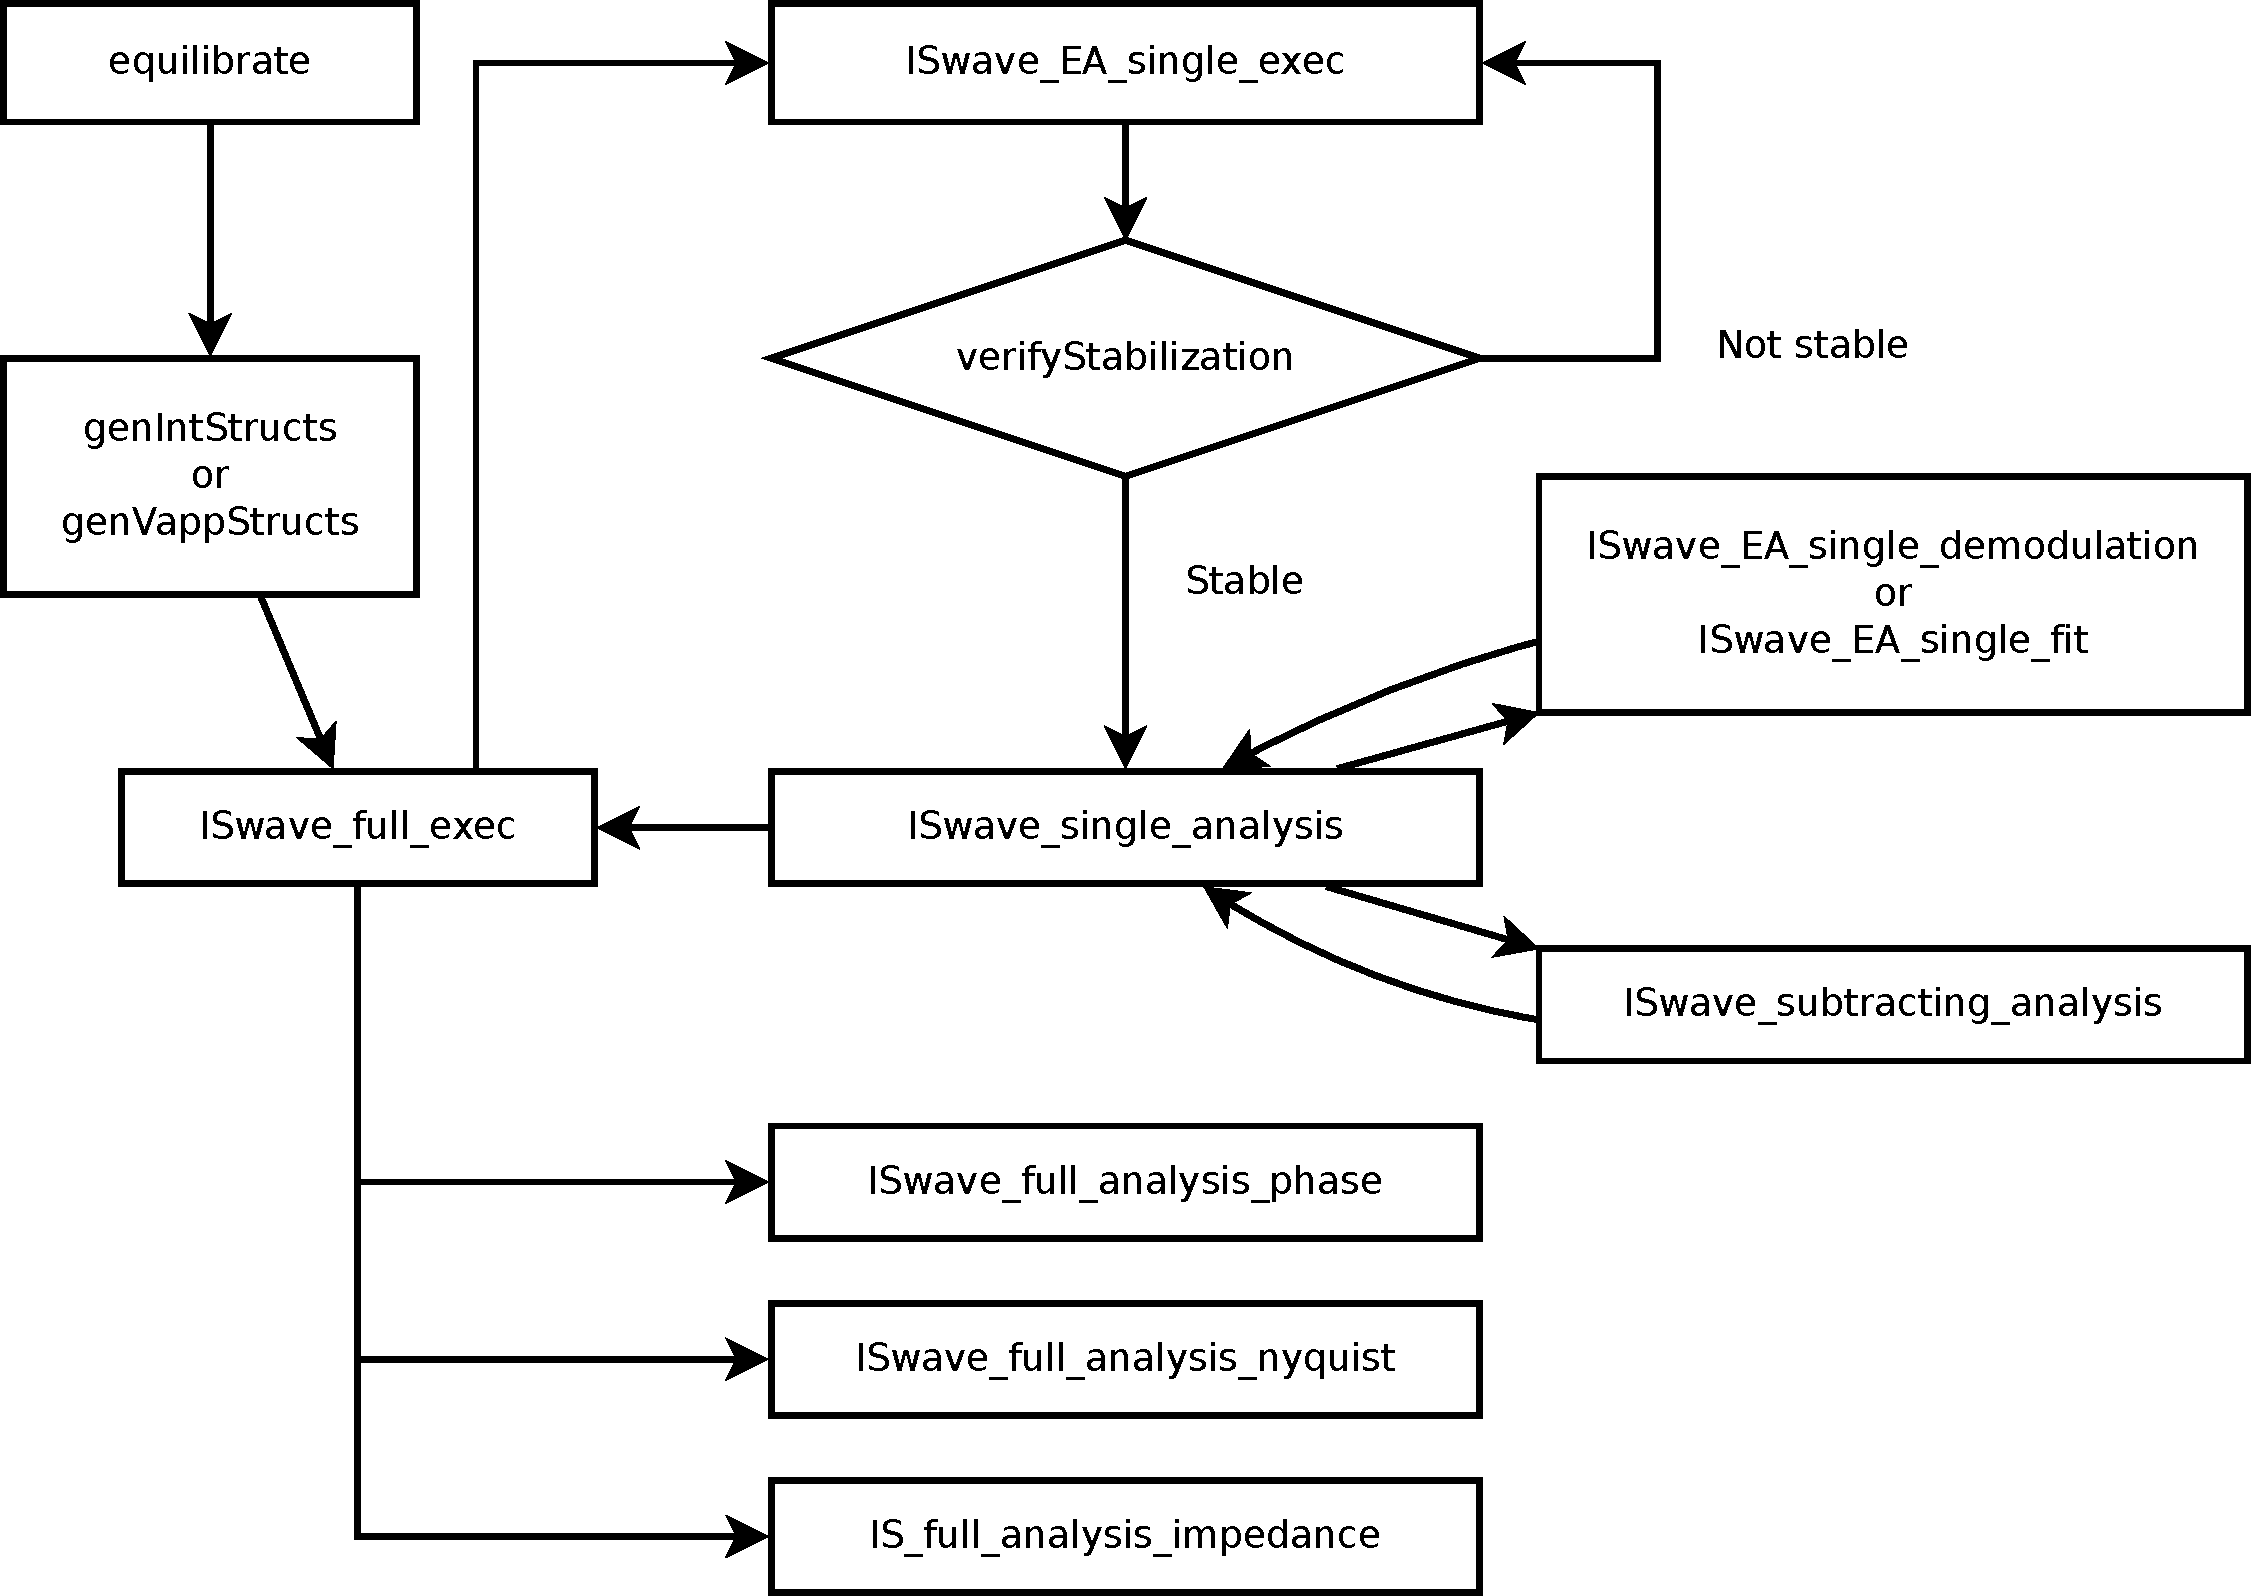
\includegraphics[width=1.05\textwidth]{flowchart/flowchart-crop.pdf}
		\mycaption[Flowchart of impedance simulation modules.]{
			The representation indicates the logical flow of the simulation, in some parts does not corresponds to the actual calls.
			Also, some of the secondary pieces have been skipped for simplicity.
			\texttt{equilibrate} is part of Driftfusion core and generates stabilised solutions, while \texttt{gen\-Int\-Structs}, \texttt{gen\-Vapp\-Structs}, and \texttt{verify\-Stabilization} are described in \cpageref{verifyStabilization,genVappStructs}.
		}\label{fig:impedance_flowchart}
	\end{figure}

	I choose to split the implementation in independent modules, so that some of them can be easily re-used for other kinds of simulations.
	The logical flowchart of a complete impedance spectra simulation has been represented in \cref{fig:impedance_flowchart}.


	\paragraph{\texttt{ISwave\_EA\_single\_exec} -- Does a single impedance spectroscopy simulation}
	Starting from the last time point of the provided solution it applies a time-varying voltage.
	This voltage profile is the background voltage bias from the provided solution summed to a sinusoidally oscillating voltage.

	\textit{Inputs:} 1) a single asymmetric structure as created by \texttt{pindrift};
	2) voltage oscillation amplitude in volts;
	3) voltage oscillation frequency;
	4) number of periods to be simulated;
	5) how many time points should the solution have for
	each period, suggested to use a multiple of 4;
	6) logical, check if the oscillating solution reached a
	(oscillating) stabilization, otherwise just use the result of the
	initial simulation. This can be useful when it's known that the
	starting solution is not stabilized, for example measuring with an
	unstabilized ionic profile;
	7) logical, set to true when performing ElectroAbsorbance simulation,
	this will skip the electrical current calculation;
	8) starting relative tolerance of the \texttt{pdepe} solver, for example a
	value of \num{1e-8} sets for a very precise simulation.

	\textit{Outputs:} a structure with a solution being perturbed by an
	oscillating voltage.

	\textit{Requires:} \texttt{pindrift}, \texttt{verify\-Stabilization}, \texttt{pinana}.

	\textit{Required by:}

	\textit{Example:} using \texttt{asymmetricize} (see \cpageref{asymmetricize}) the symmetric solution at 1 sun illumination and open circuit is broken in halves in order to be able to apply a custom voltage.
	Then this script simulates an oscillating voltage at \SI{0.1}{\Hz} and \SI{2}{\mV} of half peak to peak voltage amplitude, with a constant voltage bias equal to the device \gls{voc},
	20 periods and 40 time points per period, taking care of reaching a stable solution,
	and using a starting relative tolerance of \num{1e-8} and calculates also the electronic current needed by impedance simulations.
	\begin{lstlisting}[style=Matlab-editor]
>> asymssol_i_1S_SR_is_100mHz_2mV = ISwave_EA_single_exec(asymmetricize(ssol_i_1S_SR), 2e-3, 1e-2, 20, 40, true, false, 1e-8)
   \end{lstlisting}

	\paragraph{\texttt{ISwave\_EA\_single\_demodulation} -- Calculates phase and amplitude demodulating oscillating current data from impedance spectroscopy}\label{ISwave_EA_single_demodulation}
	The current profile gets multiplied by the voltage profile and,
	separately, by the voltage profile with an additional 90 degrees phase.
	The integrals of the resulting profiles are related to the phase.
	This simulates the working principle of a dual-phase demodulator often
	used by lock-in amplifiers.
	A phase close to \SI{90}{\degree} results in very small values of
	the in-phase integral which can have a wrong sign and result in a wrong phase of
	\SI{-90}{\degree}, in that case the simulation should be repeated with smaller \texttt{pdepe}
	relative tolerance.

	\textit{Inputs:} 1) a column with the time mesh;
	2) a column with the value to be fitted, which in case of impedance simulation is the current \textsl{versus} time profile;
	3) an anonymous function containing a constant bias, the amplitude of
	the sinusoid, its phase and the frequency;
	4) an array with the parameters used for calculating the applied
	oscillating voltage in the provided anonymous function.

	\textit{Outputs:} an array with the values from the demodulation: constant
	bias, sinusoid amplitude, phase shift.

	%		\textit{Requires:} 

	\textit{Required by:}


	\textit{Example:} demodulate the components of the oscillating current.
	\begin{lstlisting}[style=Matlab-editor]
>> ISwave_EA_single_demodulation(asymssol_i_1S_SR_is_100mHz_2mV.t', asymssol_i_1S_SR_is_100mHz_2mV.Jn, @(coeff, t) coeff(1) + coeff(2) * sin(coeff(3) + coeff(4) * t), asymssol_i_1S_SR_is_100mHz_2mV.p.Vapp_params)
		\end{lstlisting}


	\paragraph{\texttt{ISwave\_EA\_single\_fit} -- Calculates phase and amplitude fitting oscillating current data from impedance spectroscopy}
	This is an alternative to \texttt{ISwave\_EA\_single\_demodulation} which can be used to confirm the demodulation results.

	\textit{Inputs:} 1) an array with the time mesh;
	2) an array with the value to be fitted, which in case of impedance simulation is the current \textsl{versus} time profile;
	3) an anonymous function to be used for the fitting, containing
	a constant bias, the amplitude of the sinusoid and its phase. The
	frequency is taken as it is from input, it is not fitted.

	\textit{Outputs:} an array with the values from the sinusoidal fit: constant
	bias, sinusoid amplitude, phase shift.

	%\textit{Requires:} 

	\textit{Required by:}

	\textit{Example:} fits the oscillating current \textsl{versus} voltage data for a \SI{200}{\Hz} simulation.
	\begin{lstlisting}[style=Matlab-editor]
>> ISwave_EA_single_fit(asymssol_i_1S_SR_is_100mHz_2mV.t, asymssol_i_1S_SR_is_100mHz_2mV.Jn, @(coeff, t) coeff(1) + coeff(2) * sin(coeff(3) + 2 * pi * 200 * t))
\end{lstlisting}



	\paragraph{\texttt{ISwave\_single\_analysis} -- Calculate impedance and phase from impedance spectroscopy data}
	The imaginary and real components of complex impedance (respectively reactance and resistance) are extracted using either \texttt{ISwave\_EA\_single\_demodulation} or \texttt{ISwave\_EA\_single\_fit}.

	\textit{Inputs:} 1) a structure with a solution being perturbed by an
	oscillating voltage, as generated from \texttt{ISwave\_EA\_single\_exec};
	2) logical, when true graphics does not get created and
	\texttt{ISwave\_subtracting\_analysis} does not get launched, useful when
	launched under parallelization;
	3) logical, get phase via demodulation instead of using a fitting.

	\textit{Outputs:} 1) array of background current, half peak to peak amplitude of
	oscillation and phase of total electronic current;
	2) array of background current, half peak to peak amplitude of
	oscillation and phase of ionic displacement current;
	3) array of background current, half peak to peak amplitude of
	oscillation and phase of recombinating charge per unit time;
	4) array of background current, half peak to peak amplitude of
	oscillation and phase of accumulating current, this is the real
	capacitive current, obtained comparing the free charges profiles at
	different times;
	5) array of background current, half peak to peak amplitude of
	oscillation and phase of non ionic current as obtained via
	subtraction of ionic current from total electronic current.

	\textit{Requires:} \texttt{ISwave\_subtracting\_analysis}, \texttt{ISwave\_EA\_single\_fit}, \texttt{ISwave\_EA\_single\_demodulation}, \texttt{pinana}.

	\textit{Required by:}

	\textit{Example:} plot current profile, reference profiles and calculate the phase using demodulation approach.
	\begin{lstlisting}[style=Matlab-editor]
>> ISwave_single_analysis(asymssol_i_1S_SR_is_100mHz_2mV, false, true)
\end{lstlisting}

	\paragraph{\texttt{ISwave\_subtracting\_analysis} -- Calculates the time derivative of the total charge in the device}
	The charge excess in a device compared with the previous time point gets expressed as a current.
	This is used as a reference for impedance spectroscopy and for separating the ionic contribution.

	\textit{Inputs:} a structure with a solution being perturbed by an
	oscillating voltage, as generated from \texttt{ISwave\_EA\_single\_exec}.

	\textit{Outputs:} 1) charge variation over time in the whole device;
	2) charge variation over time in the perovskite layer.

	%\textit{Requires:} 

	\textit{Required by:}

	\textit{Example:} extract reference values.
	\begin{lstlisting}[style=Matlab-editor]
>> [subtracting_n_t, subtracting_n_intr_t] = ISwave_subtracting_analysis(asymssol_i_1S_SR_is_100mHz_2mV)
\end{lstlisting}

	\paragraph{\texttt{ISwave\_full\_exec} -- Simulates impedance spectroscopy at various frequencies on many provided solutions}
	A single structure can be provided as steady state solution to start from for simulating impedance spectroscopy.
	Alternatively, a cell containing various structures can be provided.
	For example, if a cell generated using \texttt{gen\-Int\-Structs} (see \cpageref{genIntStructs}) is provided, the impedance at various light intensities can be compared.
	Or, if the provided cell has been generated using \texttt{gen\-Vapp\-Structs} (see \cpageref{genVappStructs}), solutions with different background voltage bias can be compared.
	If Matlab's Parallel Computing Toolbox is available, this scripts runs in parallel on all the available physical CPU cores, otherwise it just runs on one core.

	\textit{Inputs:} 1) can be a cell structure containing either symmetrical or asymmetrical structures. Various background
	light intensities can be provided using \texttt{gen\-Int\-Structs} and various applied voltages using \texttt{gen\-Vapp\-Structs}.
	Otherwise it can be a single structure as created by \texttt{pindrift};
	2) highest frequency limit;
	3) lowest frequency limit;
	4) number of points to simulate between the lowest and
	the highest frequency;
	5) voltage oscillation amplitude in volts, \SI{1}{\mV} should be enough but larger values can be employed for reducing the noise or having a large perturbation simulation;
	6) logical, after stabilization sets the mobility of
	ionic defects to zero to simulate the impedance with effectively frozen ions;
	7) logical, determines which method to use for extracting phase and amplitude of the current.
	If false, always uses fitting \textsl{via} \texttt{ISwave\_EA\_single\_fit}, if true uses demodulation \textsl{via} \texttt{ISwave\_EA\_single\_demodulation}. Anyway if the obtained phase is weird, fit will be used
	automatically for confirming the result;
	8) logical, whether to graph the individual solutions and
	the overall graphics.

	\textit{Outputs:} a structure containing the most important results of the simulation.

	\textit{Requires:} \texttt{asymmetricize}, \texttt{ISwave\_EA\_single\_exec},
	\texttt{ISwave\_single\_analysis}, \texttt{ISwave\_full\_analysis\_nyquist},
	\texttt{IS\_full\_analysis\_impedance}, \texttt{ISwave\_full\_analysis\_phase}, \texttt{pinana},
	\texttt{stabilize}.

	%\textit{Required by:} 

	\textit{Example:} This is the most typical of the performed simulations: calculate on 8 different illumination intensities including dark, do not freeze ions, use a half peak to peak
	voltage oscillation amplitude of 2 mV, on 23 points from frequencies of 1 GHz to
	0.01 Hz and plot all graphics, including the ones for each solution.
	\begin{lstlisting}[style=Matlab-editor]
>> ISwave_oc = ISwave_full_exec(genIntStructs(ssol_i_eq_SR, 1, 1e-3, 7, true), 1e9, 1e-2, 56, 2e-3, false, true, true)
\end{lstlisting}

	\paragraph{\texttt{ISwave\_full\_exec\_nonparallel} -- Non parallelized version of \texttt{ISwave\_full\_exec}}
	The fundamental difference from \texttt{ISwave\_full\_exec} is the lack of \texttt{parfor}
	for parallel computation. This allows more flexibility at the cost of a
	more time demanding simulation.

	\textit{Inputs:} 1-5) identical to \texttt{ISwave\_full\_exec} 1-5 ones;
	6) logical, if true do not check that the oscillating solution reached a
	(oscillating) stabilization, instead take always the first solution
	and use its final time point as the starting point of the next
	frequency simulation. This can be useful when it's known that the
	starting solution is not stabilized and a realistic simulation of the
	solution evolving during the measurement is wanted.
	7-9) identical to \texttt{ISwave\_full\_exec} 6-8 ones;
	10) logic, defines whether to save in volatile base
	workspace each of the calculated solutions.

	\textit{Outputs:} a structure containing the most important results of the simulation.

	\textit{Requires:} \texttt{asymmetricize}, \texttt{ISwave\_EA\_single\_exec},
	\texttt{ISwave\_single\_analysis}, \texttt{ISwave\_full\_analysis\_nyquist},
	\texttt{IS\_full\_analysis\_impedance}, \texttt{ISwave\_full\_analysis\_phase}, \texttt{pinana},
	\texttt{stabilize}.

	%\textit{Required by:} 

	\textit{Example:} Identical to the example shown for \texttt{ISwave\_full\_exec} but this also saves to base workspace the single oscillating solutions and starts each simulation from the last time point of the previous, strictly sequentially without reaching stabilization.
	\begin{lstlisting}[style=Matlab-editor]
>> ISwave_oc_sequential = ISwave_full_exec_nonparallel(genIntStructs(ssol_i_eq_SR, 1, 1e-3, 7, true), 1e9, 1e-2, 56, 2e-3, true, false, true, true, true)
\end{lstlisting}

	\paragraph{\texttt{ISwave\_full\_analysis\_phase} -- Represents Bode plots of phase from impedance spectroscopy}
	The phase of the current oscillation with regards to the applied voltage is plotted as obtained from simulations made with \texttt{ISwave\_full\_exec} or \texttt{ISwave\_full\_exec\_nonparallel}.


	\textit{Inputs:} a structure containing the most important results of the simulation.

	%		\textit{Outputs:} 

	%		\textit{Requires:} 

	\textit{Required by:}


	\textit{Example:} do phase Bode plots.
	\begin{lstlisting}[style=Matlab-editor]
>> ISwave_full_analysis_phase(ISwave_oc)
				\end{lstlisting}

	\paragraph{\texttt{IS\_full\_analysis\_impedance} -- Represents Bode plots of impedance and apparent capacitance from impedance spectroscopy}
	Plot the value of absolute impedance magnitude $|Z|$, resistance $Z'$ (real component), reactance $Z''$ (imaginary component), and apparent capacitance defined as $\omega^{-1}\Im(Z^{-1})$ at various frequencies and various illumination or background voltage bias conditions.
	As a reference, the following currents are also used for plotting the mentioned quantities: ionic displacement current, recombination current, and total charge time derivative as obtained from \texttt{ISwave\_subtracting\_analysis}.

	\textit{Inputs:} a structure containing the most important results of the simulation.

	%\textit{Outputs:} 

	%\textit{Requires:} 

	\textit{Required by:}

	\textit{Example:} do impedance and apparent capacitance Bode plots.
	\begin{lstlisting}[style=Matlab-editor]
>> IS_full_analysis_impedance(ISwave_oc)
\end{lstlisting}

	\paragraph{\texttt{ISwave\_full\_analysis\_nyquist} -- Plots Nyquist graph for impedance spectroscopy}
	Nyquist plot refers the imaginary component of the impedance to its real component.
	A normalized spectra is also plotted and the rescaling factors are indicated in the legend.

	\textit{Inputs:} a structure containing the most important results of the simulation.

	%\textit{Outputs:} 

	%\textit{Requires:} 

	\textit{Required by:}

	\textit{Example:} do Nyquist plot.
	\begin{lstlisting}[style=Matlab-editor]
>> ISwave_full_analysis_nyquist(ISwave_oc)
\end{lstlisting}




	\paragraph{\texttt{from\-ISwaveEA\-Struct\-ToTxt} -- Exports single impedance simulation data to text files}
	This helper saves the main data from a oscillating solution created by \texttt{ISwave\_EA\_single\_exec} to text files, for easing the import with Origin (from OriginLab).

	\textit{Inputs:} 1) a structure with a solution being perturbed by an oscillating voltage, as generated from \texttt{ISwave\_EA\_single\_exec};
	2) char array, prefix to be used for the text files names.

	%\textit{Outputs:} 

	%\textit{Requires:} 

	%\textit{Required by:} 

	\textit{Example:} save single simulation data to text files.
	\begin{lstlisting}[style=Matlab-editor]
>> fromISwaveEAStructToTxt(asymssol_i_1S_SR_is_100mHz_2mV, 'asymssol_i_1S_SR_is_100mHz_2mV')
\end{lstlisting}

	\paragraph{\texttt{from\-ISwave\-Results\-ToTxt} -- Exports data of a set of impedance simulations to text files}
	This helper saves the main data from a complete impedance spectroscopy simulation including various solutions created by \texttt{ISwave\_full\_exec} to text files, for easing the import with Origin (from OriginLab).

	\textit{Inputs:} 1) a structure containing the most important results of the simulation;
	2) char array, prefix to be used for the text files names.

	%\textit{Outputs:} 

	%\textit{Requires:} 

	%\textit{Required by:} 

	\textit{Example:} save data from a set of simulations to text files.
	\begin{lstlisting}[style=Matlab-editor]
>> fromISwaveResultsToTxt(ISwave_oc, 'ISwave_oc')
\end{lstlisting}


\section{Further development}


	\begin{figure}
		\makebox[\textwidth][c]{
			\parbox{1.1\textwidth}{
				\centering
				\begin{subfigure}[t]{1.1\textwidth}
					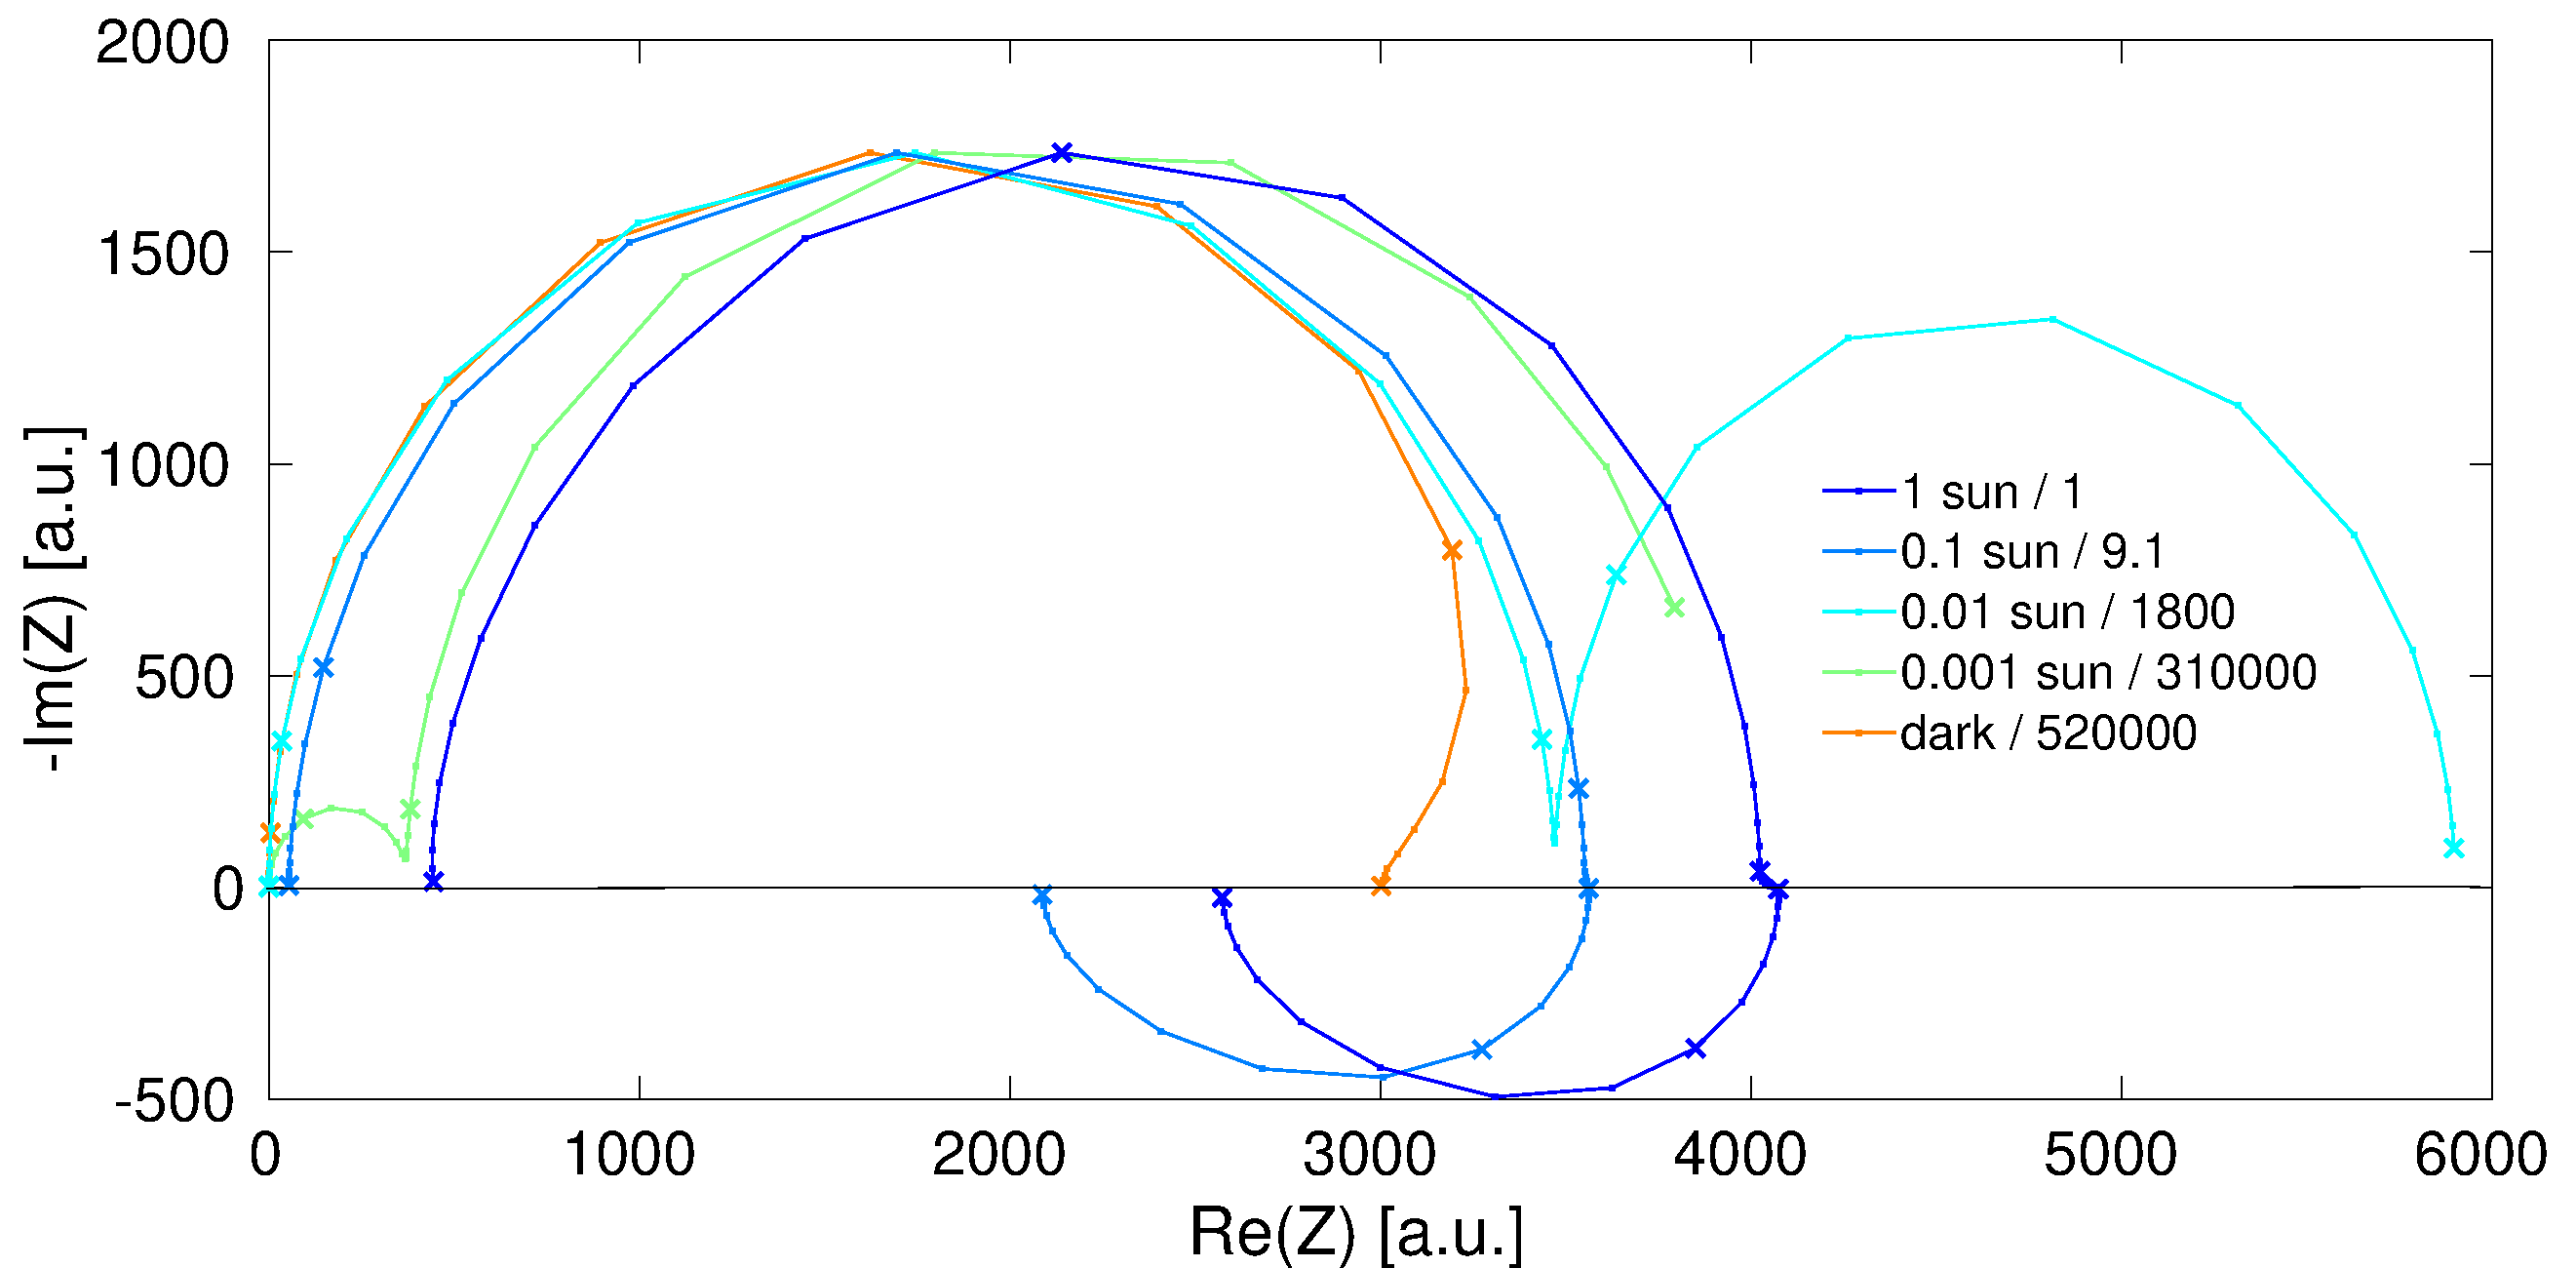
\includegraphics[width=1\textwidth]{heterojunction/ISwave_oc_nyquist_norm.png}
					\subcaption{Illuminated, open circuit, Nyquist}\label{fig:impedance_heterojunction-oc-nyquist}
				\end{subfigure}
				%			\qquad
				\bigskip

				\begin{subfigure}[t]{1.1\textwidth}
					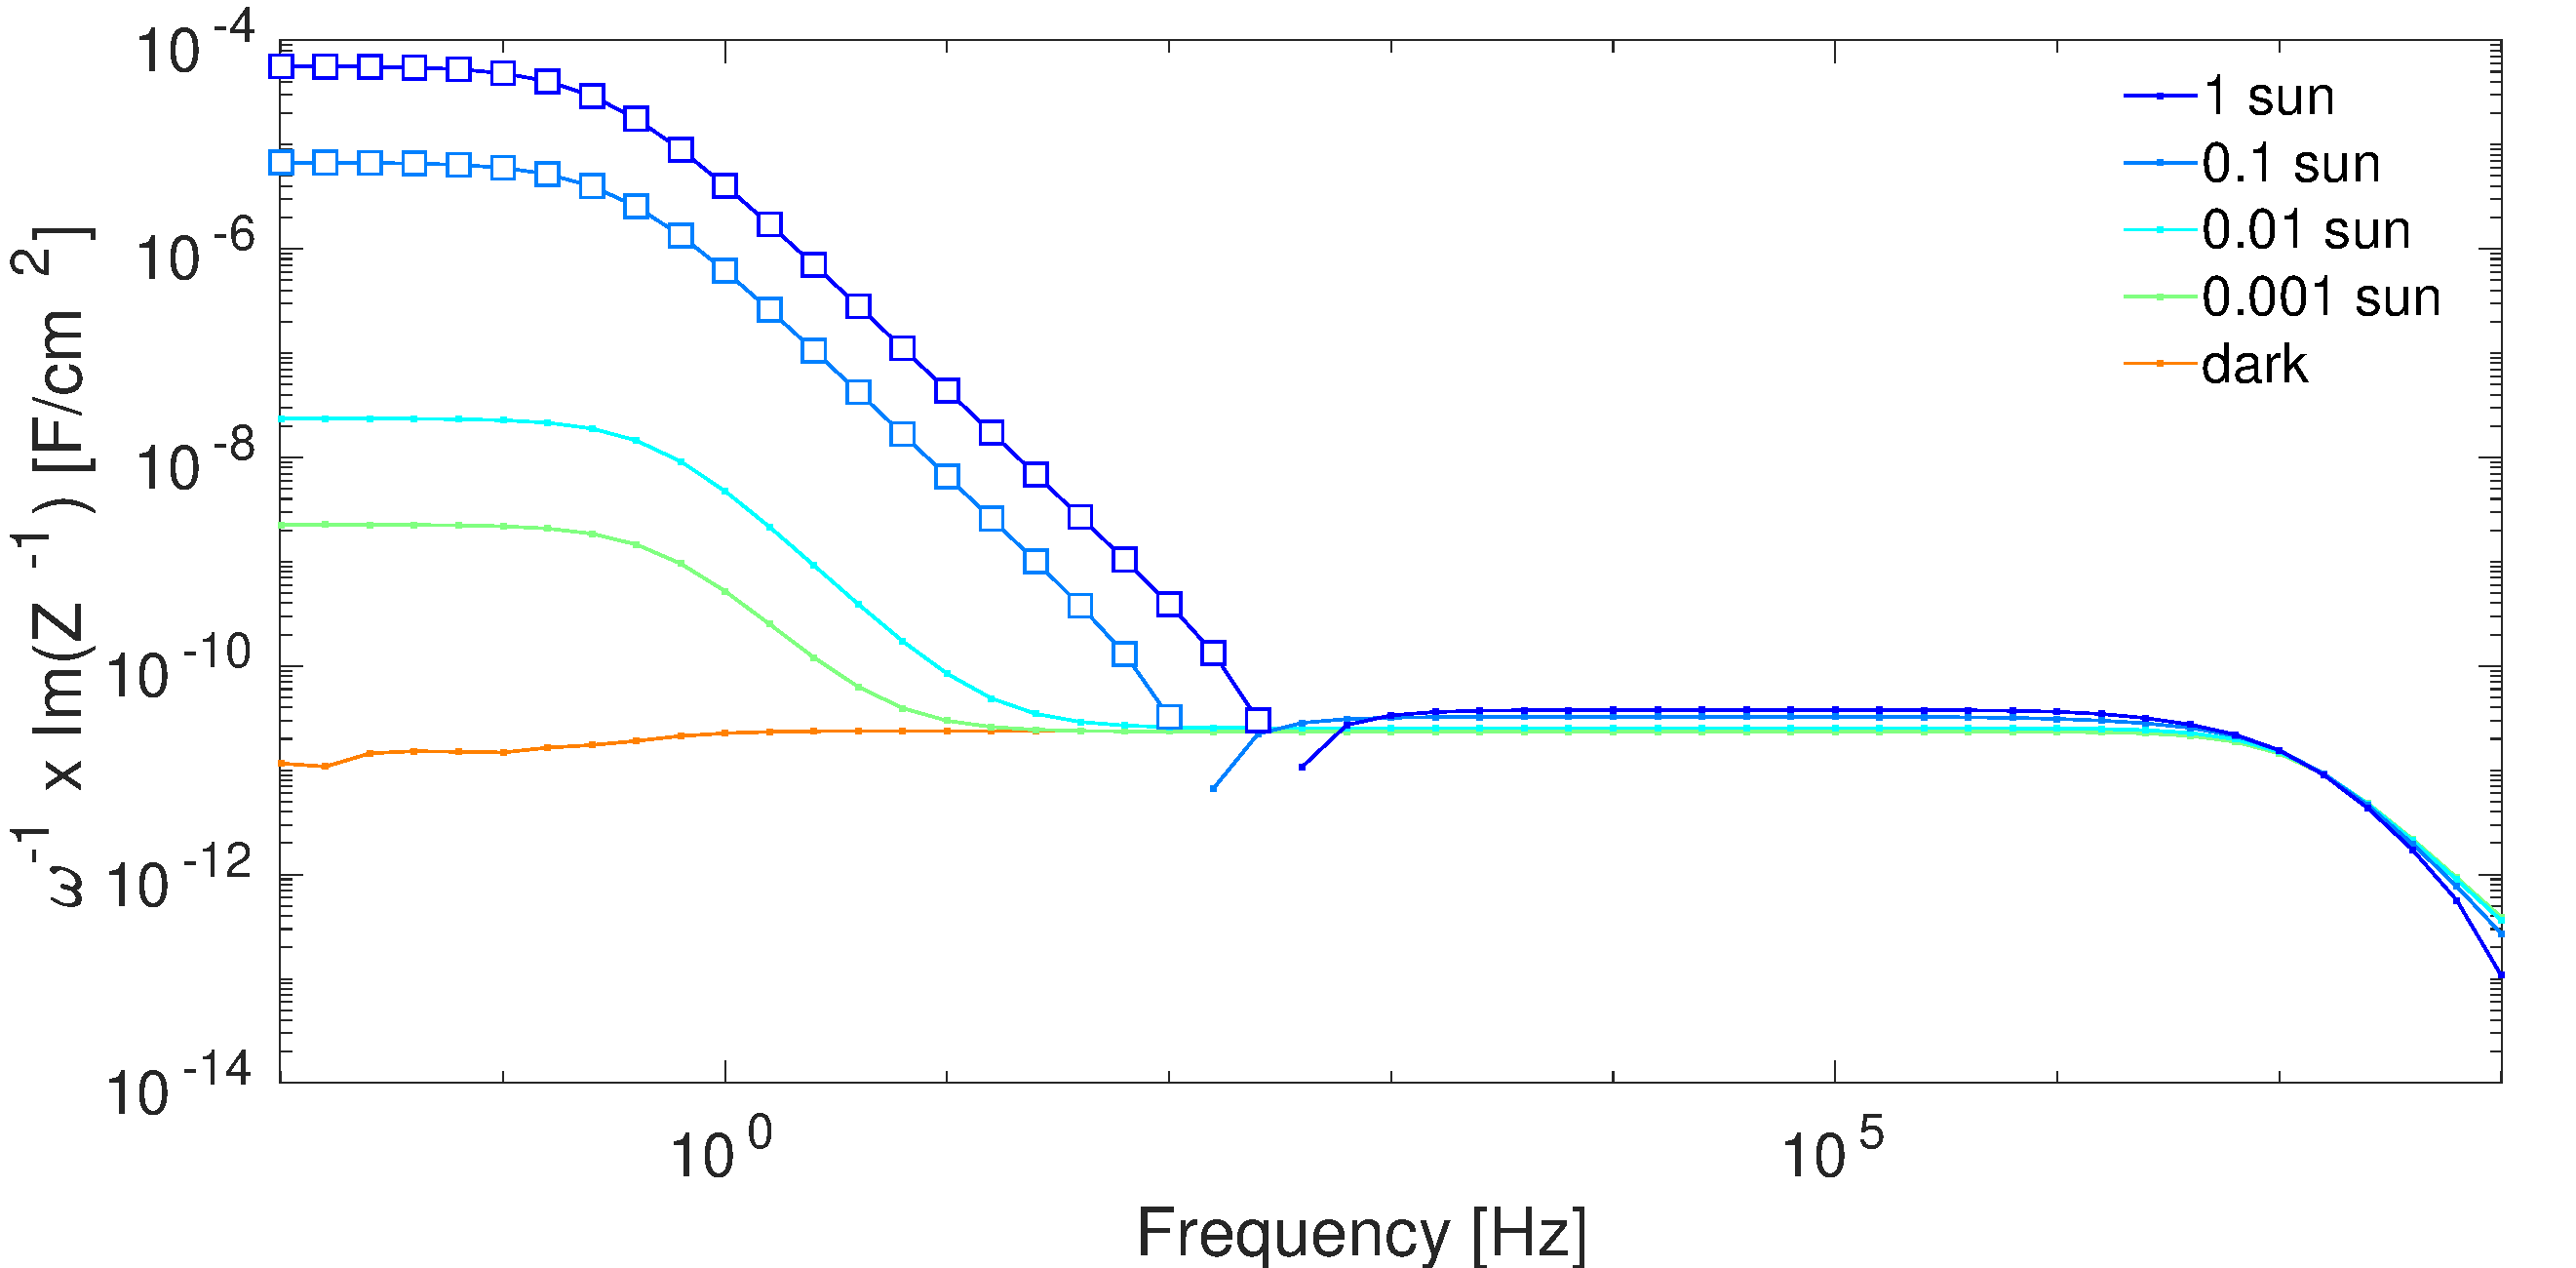
\includegraphics[width=1\textwidth]{heterojunction/ISwave_oc_cap.png}
					\subcaption{Illuminated, open circuit, apparent capacitance}\label{fig:impedance_heterojunction-oc-cap}
				\end{subfigure}
				%			\bigskip
				%			
				%			\begin{subfigure}[t]{0.51\textwidth}
				%				\includegraphics[width=1\textwidth]{heterojunction/ISwave_Vapp_nyquist_norm.png}
				%				\subcaption{Dark, applied voltage, Nyquist}\label{fig:impedance_heterojunction-vapp-nyquist}
				%			\end{subfigure}
				%						\qquad
				%			\begin{subfigure}[t]{0.51\textwidth}
				%				\includegraphics[width=1\textwidth]{heterojunction/ISwave_Vapp_cap.png}
				%				\subcaption{Dark, applied voltage, apparent capacitance}\label{fig:impedance_heterojunction-vapp-cap}
				%			\end{subfigure}
				\mycaption[Preliminary simulations of impedance on heterojunction model.]{The filled symbols indicate positive capacitance values, the hollow symbols represents negative capacitance which was changed in sign in order to be plotted on the same axis.}\label{fig:impedance_heterojunction}
			}
		}
	\end{figure}


	\paragraph{Heterojunction}
	The simulations shown here are all based on a p-i-n homojunction model, so a proper injection barrier could not actually be simulated and the negative capacitance has been obtained playing with extreme values of other parameters as aforementioned.
	An attempt of adapting the impedance scripts to the most recent heterojunction version of Driftfusion confirmed the presence of negative capacitance due to injection barrier modulation by ionic charge, as shown in \cref{fig:impedance_heterojunction}.
	Further work is needed for completely adapting the impedance scripts to the upstream heterojunction core code.

	\paragraph{Implement other similar techniques}
	We refer with the names of ElectroAbsorbance or Stark spectroscopy to the absorbance variation caused by an oscillating applied voltage.
	This effect stems from the higher absorptivity of a material in presence of an electric field.
	This simulation has already been implemented but the code release is waiting for the publication of the related work; the description of the modules is already available in \cpageref{software_electroabsorbance}.
	Using some of the modules already implemented for impedance spectroscopy simulation, it should be easy to implement also other characterization techniques like Intensity-Modulated Photovoltage/Photocurrent Spectroscopy (IMVS, IMPS) \cite{Pockett2015,Guillen2014} and Mott-Schottky capacitance analysis \cite{Almora2016}.



